\documentclass[
  manuscript=article,
  layout=preprint,
  year=2026,
  volume=x,
]{extra/joas}

% THE PAPER'S SOURCE. Check its numbers with: python3 scripts/paper_claims.py check analysis/joas/main.tex

\doi{xx.xxxxx/joas.xxxx.xxxx}

\received {1 April 20xx}
\revised  {1 May 20xx}
\accepted {10 May 20xx}
\published{20 May 20xx}

\editor{Editor Name}

\reviewers{First Reviewer, Second Reviewer, Third Reviewer}

\addbibresource{reference.bib}

% Long \texttt file names cannot hyphenate in typewriter font; let them break, and let TeX stretch interword
% space in a paragraph it cannot break rather than overflow into the margin.
\usepackage[htt]{hyphenat}
\hypersetup{pdftitle={Taxi-out Time as a Database Record}, pdfauthor={Arquimedes Canedo}}
\setlength{\emergencystretch}{3em}
% The class paints every table row white with zero rule spacing (\patchCUPtables). Preview and other Core Graphics
% viewers then draw the white header cells over the top rule, on some tables and not others. Plain booktabs instead.
\renewcommand{\patchCUPtables}{}
\usepackage{tabularx}
% Pale tints of the figures' two hues (scripts/fig_palette.py), as cell backgrounds for the few table cells the prose
% singles out: the record, the measurement. Backgrounds, not text colour, so they survive printing in black and white.
\definecolor{recordtint}{HTML}{EFC6B6}
\definecolor{measuredtint}{HTML}{C2D0E5}

\title{Taxi-out Time as a Database Record}

\author{Arquimedes Canedo \orcid{0000-0003-3506-6563}}
\affiliation{Independent Researcher, Princeton, NJ, USA}
\email{canedo@sector.mx}

\keywords{taxi-out time; airport operational data; data quality; ADS-B; machine learning}

\abbreviations{
    ADS-B: Automatic Dependent Surveillance-Broadcast,
    RMSE: root mean squared error
}

\begin{document}

\begin{abstract}
In airport operational data, a departure's taxi-out time is its take-off time minus the off-block time the airport recorded, and the recorded off-block is whatever the airport's system wrote. We study a year of such records at ten large European airports and find that the target is a database record rather than a measurement. Four aircraft had not yet landed when their record says they left the stand. Among the recorded taxis of two hours or more that can be chained to the aircraft's previous arrival, a third exceed the time between that arrival and the take-off, which no taxi can. One airport writes the scheduled time when it has no off-block. The model is built on this reading. Where the airport captured a real pushback, the record is the pushback and an open sensor can measure it: a trajectory stage on raw ADS-B surface tracks from the adsb.lol archive learns when to trust them. Where it did not, the file shows how the record was written: a carrier's failing data feed is read from the arrivals of the scored months, which keep their labels, and the flight-plan join, which succeeds only within an hour of the recorded off-block, bounds the hidden off-block. These two halves sit on a base model, a blend of nine regression members followed by a mixture over the values a record can hold. The mechanisms were found by studying the errors of a model built for the competition, and each enters the final model as a rule whose evidence is labelled; the final model carries no value fitted to a leaderboard score. On the January and July 2026 departures it scores 233.75 s RMSE, against 292.05 s for its base without trajectory data or rules, and the same code predicted February and June 2026, added by the organisers at the close, without feedback. The version entered during the competition also carried constants fitted to leaderboard scores and scored 222.85 s; those constants are disclosed, and that score is not a measure of the method. The scored months were evaluated repeatedly, which Section~\ref{sec:8} discusses. Records of this kind also feed the European indicator of additional taxi-out time.
\end{abstract}

\section{Introduction}\label{sec:1}

A taxi-out time is the interval between an aircraft leaving its stand and taking off. In the operational data airports keep, that interval is not observed directly. A system writes an off-block time into a database and a take-off time beside it, and the taxi-out time is the difference between the two entries. When the system holds an off-block it actually captured, the difference is the taxi. When it does not, the system writes something else, and the difference is whatever that entry implies. At Rome Fiumicino the something else is the scheduled off-block time. A flight that pushed back hours late is then recorded as a flight that taxied for hours, and four aircraft in this dataset had not yet landed when their record says they left the stand.

The consequence reaches beyond prediction. The European indicator of additional taxi-out time is computed from the off-block and take-off times airports report~\cite{eurocontrol_atxot2023}. Taxi-out time is also a planning input for airport collaborative decision making~\cite{eurocontrol_acdm} and an input to fuel and emission estimates. Each of these inherits whatever the recording system wrote.

This paper studies a year of such records at ten large European airports, the data of the EUROCONTROL PRC Data Challenge 2026: 2,085,047 departures in 2025 with their taxi-out time given, and 344,841 departures in January and July 2026 whose recorded off-block is withheld and whose taxi-out time is to be predicted under a squared-error loss. At the close the organisers added 325,949 departures of February and June 2026, predicted without feedback.

Our thesis is that the target is a record, and that reading it as one tells a model where to measure and where to reconstruct. Where an airport captured a real pushback, its record is the pushback, and a sensor that watched the aircraft can measure it. Where it did not, no sensor can help, because the value to predict is what the system wrote in place of a pushback; the file itself, however, shows how that value was written, and a rule can reconstruct it. The two cases call for different methods, and the largest errors belong to the second. Those errors are a property of the recording systems, and the remedy for them lies there rather than in a better model.

The paper makes four contributions:

\begin{enumerate}
\item a characterisation of the target as a record, airport by airport (Section~\ref{sec:4});
\item a trajectory stage that measures the pushback from raw ADS-B surface tracks where the record is a real pushback (Section~\ref{sec:5.2});
\item rules that reconstruct the record where it is not, from a carrier's failing data feed and from the flight-plan join (Section~\ref{sec:5.3});
\item a final model with no value fitted to a score on the scored months, its score there predicted before its one submission, and two further months predicted without feedback (Section~\ref{sec:7}).
\end{enumerate}

The trajectory stage and the rules sit on a base model. The base model is a weighted average of nine regression models, each trained to predict an ordinary taxi time; the paper calls the average the \textbf{blend} and the models its \textbf{members}. A mixture step follows: for a row whose record is not a taxi at all, the mixture can replace the regression's estimate with a timestamp copied from another column of the same record, the scheduled off-block for example. The trajectory stage acts on the rows the sensor covers and never overrides the mixture. The rules act where the record was written from something other than a pushback, which is mostly one airport; there, on the rows where the labelled year makes a schedule copy about as likely as a taxi, a classifier re-weights the two.

The work proceeded in two stages, and the paper reports both. The first built the strongest model we could for the competition, the \textbf{competition model}, and studied its errors; that is how the mechanisms of Section~\ref{sec:4} were found. Reading its largest residuals row by row exposed Fiumicino's schedule copies and date errors (Sections~\ref{sec:4.4} and~\ref{sec:4.5}). A search over labelled 2025 data in the groups of Fiumicino rows whose predictions it had replaced outright with the schedule copy, and its January errors, led to carriers whose data feed fails (Section~\ref{sec:4.6}). And a separate AI agent session, given the challenge's files and its predictions, found the flight-plan join (Section~\ref{sec:4.7}). The version entered on the leaderboard also carried constants fitted to its returned scores; they are disclosed in Section~\ref{sec:5.1} and discussed in Section~\ref{sec:8}.

The second stage built the \textbf{final model}: the same design, keeping each mechanism as a rule whose evidence is labelled 2025 data or the labelled arrivals of the scored months, with no value fitted to a score. It is retrained once and predicts four months: January and July against a score predicted before submission, February and June without feedback (Section~\ref{sec:7}). On January and July the final model scores 233.75 s and the competition model 222.85 s. The competition model's score includes the fitted values, so the final model's is the one that measures the method, and it is the model this paper reports.

\section{Related work}\label{sec:2}

Taxi-out prediction is usually posed as estimating how long an aircraft takes from pushback to take-off, with queueing, simulation, regression and learning models~\cite{balakrishna2010accuracy,ravizza2013combined,herrema2018taxi}. Where surface surveillance exists it has been used to predict departure taxi times~\cite{srivastava2011improving,levy2008departure} and compared with reported times for taxi-out benchmarking~\cite{hotle2016using}, although such surveillance covers an aircraft only once it enters the movement area, not at the stand~\cite{hotle2016using}. Taxi events and pushbacks can be extracted from surveillance and ADS-B tracks~\cite{mirmohammadsadeghi2020taxi,stloukal2026analyzing,schultz2020analysis}, with open tooling for trajectory processing~\cite{olive2019traffic} and an open receiver network behind much of it~\cite{schafer2014bringing}. Most of this work takes the recorded off-block as the physical one, or measures the movement that follows it.

The records themselves have received less attention. Airport Collaborative Decision Making defines the milestones this dataset records, among them the target off-block time, the actual off-block time and the estimated taxi-out time (TOBT, AOBT, EXOT)~\cite{eurocontrol_acdm}, and flight-plan messages exchanged under ICAO procedures carry the planned and actual times the network sees~\cite{icao_doc4444}. The documentation of the European indicator of additional taxi-out time names the precision of the reported off-block as key~\cite{eurocontrol_atxot2023}. Airline-reported gate-out times have been compared with surface radar before~\cite{signor2006accurate}. Section~\ref{sec:4} shows, over a year of records at ten airports, what an airport writes when it has no off-block and how the off-block held by EUROCONTROL's Network Manager appears to be computed; Section~\ref{sec:5} shows that an open sensor recovers the off-block where the airport did capture one. Passenger-rights thresholds~\cite{ec261_2004} give operators a reason to care about recorded delay; Section~\ref{sec:4.4} finds no evidence that records are placed against them.

The data are those of the EUROCONTROL PRC Data Challenge 2026; the organisers' papers on earlier editions address take-off weight~\cite{spinielli2025takeoff} and fuel burn~\cite{sun2026fuel}. A scored set that many models are evaluated on invites overfitting to it~\cite{blum2015ladder,dwork2015reusable}, which Section~\ref{sec:8} takes up. The models here use gradient-boosted trees~\cite{ke2017lightgbm,chen2016xgboost,prokhorenkova2018catboost} and attention over neighbouring movements~\cite{vaswani2017attention}.

\section{Data and evaluation}\label{sec:3}

\textbf{Two writers, one record.} The challenge data hold departures and arrivals at ten European airports (Table~\ref{tab:2}), labelled for 2025 and scored on January and July 2026. Every row carries two records of one flight, written by two organisations. Columns suffixed \texttt{\_mvt} are written by the airport, from its own movement database. Columns suffixed \texttt{\_flt} are written by EUROCONTROL's Network Manager (NM), which holds the flight plan and the trajectories the network computes; the paper calls it the network. This paper reads the target as the first of these, and uses the second to test it.

\textbf{The target.} For a departure, \texttt{y\ =\ MVT\_TIME\ -\ BLOCK\_TIME}: the take-off time minus the airport's recorded off-block time, in seconds. A row is \textbf{extreme} when \texttt{y\ \textgreater{}=\ 7,200\ s}, a recorded taxi of two hours or more, and \textbf{ordinary} otherwise. Of the 2025 departures, 584 are extreme: Fiumicino writes 480 of them, and four airports write none (Table~\ref{tab:2}).

\begin{table}[htbp!]
  \centering
  \small
  \setlength{\tabcolsep}{5pt}\renewcommand{\arraystretch}{1.15}
  \caption{Departures by airport, 2025: most extremes are at Fiumicino.}
  \label{tab:2}
  \begin{tabular*}{\linewidth}{@{\extracolsep{\fill}}lrrrr}
  \toprule
  \textbf{Airport} & \textbf{Departures} & \textbf{Extremes} & \textbf{Per 10,000} & \textbf{Median \texttt{y} (s)} \\
  \midrule
  EDDF Frankfurt & 230,141 & 0 & 0.00 & 837 \\
  EDDM Munich & 167,334 & 0 & 0.00 & 774 \\
  EGLL London Heathrow & 239,546 & 37 & 1.54 & 1,319 \\
  EHAM Amsterdam & 247,951 & 3 & 0.12 & 742 \\
  LEBL Barcelona & 179,705 & 0 & 0.00 & 906 \\
  LEMD Madrid & 212,242 & 0 & 0.00 & 985 \\
  LFPG Paris CDG & 239,552 & 37 & 1.54 & 954 \\
  LIRF Rome Fiumicino & 160,704 & \cellcolor{recordtint}480 & \cellcolor{recordtint}29.87 & 1,025 \\
  LSZH Zurich & 134,907 & 6 & 0.44 & 711 \\
  LTFM Istanbul & 272,965 & 21 & 0.77 & 963 \\
  \midrule
  All & 2,085,047 & 584 &  &  \\
  \bottomrule
  \end{tabular*}
\end{table}

The two-hour line lies just above the 99.97th percentile of the 2025 departures (7,017 s), and above it the label behaves as a schedule copy (defined below) rather than as a long taxi: on out-of-fold 2025 predictions, the least-squares move from the regression's prediction toward the schedule copy goes all the way above two hours (a weight of 1.07) and only 0.30 of the way between one and two hours. A \textbf{day-scale} record has \texttt{y\ \textgreater{}=\ 20,000\ s}, more than five hours. That line is a reporting convention: the share of schedule copies is the same on either side of it (73.6\% below, 76.3\% above).

\textbf{The columns.} The airport's record holds \texttt{SCHED\_TIME}, \texttt{BLOCK\_TIME} and \texttt{MVT\_TIME}: the scheduled off-block, the recorded off-block and the take-off. From the network's record the paper uses \texttt{LOBT} and \texttt{IOBT}, the off-block time as last filed and as first filed in the flight plan; \texttt{EOBT\_1} and \texttt{AOBT\_3}, the estimated off-block of the flight plan and the actual off-block of the flown trajectory, the network's own account of when the aircraft left; \texttt{ARVT\_1} and \texttt{ARVT\_3}, their arrival times; and two identifiers, the airport's \texttt{FLIGHT\_ID\_mvt} and the network's \texttt{CALLSIGN\_flt}.

The \textbf{schedule deviation}, \texttt{ms\ =\ MVT\_TIME\ -\ SCHED\_TIME}, is how long after its scheduled off-block the flight took off; a record whose off-block is the scheduled time has \texttt{y} equal to \texttt{ms}. The network's implied taxi, \texttt{naive\ =\ MVT\_TIME\ -\ AOBT\_3}, is the taxi-out time the network's own off-block implies, and it is the simplest competing estimate of \texttt{y}.

A \textbf{schedule copy} is a departure whose recorded off-block lies within 60 s of its scheduled time, so that \texttt{y} equals \texttt{ms} to within a minute. The rates quoted for schedule copies use that tolerance, and a statement about exact equality says so. A schedule copy arises in two ways. A punctual pushback lands on its scheduled minute, and at most airports most schedule copies are of that kind. A \textbf{fallback} is the other kind: the airport captured no off-block and wrote the schedule in its place. A \textbf{genuine} departure is one that is not a schedule copy and whose \texttt{y} lies within 30 minutes of \texttt{naive}, so that the airport's record and the network's roughly agree on when the aircraft left.

A \textbf{cell} is the set of rows a condition picks out, for example the Fiumicino departures that failed to attach to a flight plan. The \textbf{lift} of a condition is the rate of an outcome among the rows in its cell divided by the rate over all rows, so a lift of two means the outcome is twice as common there and a lift below one means it is rarer. To \textbf{commit} a cell is to replace the model's predictions on every row of it with one hypothesis's value, for example the schedule copy.

\textbf{Two sets to score on.} The scored months are blanked, so a labelled stand-in for them is needed, and the natural one is the same two months a year earlier. The \textbf{window} is the 344,336 January and July 2025 departures with a positive target (83 of the 344,419 departures in those months have \texttt{y\ \textless{}=\ 0} and are left out): 344,187 ordinary and 149 extreme. A model evaluated on the window is trained without its months, on the ten other months of 2025; where a component needs the same season, it is fitted on one of the two months and applied to the other, which the paper calls cross-fitting (Section~\ref{sec:5.1} describes the models). Early in the work the window was scored with versions of the models that differ from those that ship; where a result rests on that earlier set-up, it is named (\ref{sec:E.1}). The \textbf{2026 set} is the 344,841 scored departures, whose labels the organisers hold; a submission returns a single number, the RMSE over all of them. It is not a clean hold-out: this work scored 90 submissions on it (Section~\ref{sec:8}). Scores on the 2026 set are reported as such, and intervals come from the window.

\textbf{Units.} Accuracy is RMSE in seconds, the root mean squared error of the predictions. Where a change has to be added up across rows, as in the oracle decompositions and the pricing identity of \ref{sec:E}, it is given as a sum of squared errors (SSE), with $\mathrm{RMSE} = \sqrt{\mathrm{SSE}/N}$ for $N$ = 344,336 on the window and 344,841 on the 2026 set. A change measured on labelled 2025 data is sometimes given in \textbf{RMSE-equivalent seconds}: the change in squared error divided by $2NR$, with $N$ the 2026 set's size and $R$ the model's RMSE level at the time of the measurement. To first order, that is the change in RMSE the same change in squared error would produce on a set of that size; it loses accuracy for large changes.

\textbf{Noise floors.} Two runs of an identical configuration that differ only in their random seeds do not score the same. Across seeds the ordinary-row window RMSE moves by 0.144 s and the extreme side by about 25 s on a 149-extreme window. Differences smaller than these are not interpreted.

\textbf{Whether the 2026 set holds a day-scale record.} A single day-scale record predicted as an ordinary taxi would carry a large share of a set's squared error (Section~\ref{sec:6.4}), so everything measured on the 2026 set depends on whether it holds one, and it appears not to. The test compares the window with the 2026 set on the same model. The window holds two day-scale rows that no observable flags (Section~\ref{sec:8}). With those two removed, and the rest reweighted to the 2026 set's composition by airport, month and flight-plan join, the window's squared error for the base model before its final blend is 2.3769e10, against the 2.2755e10 the 2026 set returned for that model: the window is 4.5\% dearer. Suppose instead that the 2026 set did hold such a row, carrying the window's 40.12\% extreme share. The returned score would then need the ordinary rows to be 21.8 to 23.4\% cheaper on the 2026 set than on the window, about four standard deviations away. The labelled year predicts 0.83 such rows in a set of this size, with a 0.44 chance of none.

\section{The taxi-out time is a record}\label{sec:4}

The target is the difference between two entries in an airport's operational database, the take-off time minus the recorded off-block, and where the record is a real pushback it is the taxi. On the rows that dominate a squared-error loss it is not, and three independent measurements show this. Among the extremes that can be chained to the aircraft's previous arrival at the same airport, 34.1\% exceed the time from that arrival to the take-off, which no taxi can, since an aircraft cannot push back before it has arrived (Section~\ref{sec:4.1}). Four extremes whose aircraft a trajectory identifies were still in the air when their record says they left the stand (Section~\ref{sec:4.2}). And a survey of the ten airports finds one writing the scheduled time into the off-block field at more than twice the rate chance produces, and no other convention for a missing off-block anywhere (Section~\ref{sec:4.4}). Sections~\ref{sec:4.3} to~\ref{sec:4.7} then read how the records are written: which system wrote each timestamp, which rows at that one airport carry the schedule, a date error and a double pushback, a carrier's failing data feed that the labelled arrivals expose, and a join rule that bounds the hidden off-block.

For a model the consequence is that physical priors work against it precisely on the largest errors. On the window the extremes are 0.0433\% of rows and carry 40.12\% of the squared error (Section~\ref{sec:6.2}); the 2026 set appears to hold no day-scale record (Section~\ref{sec:3}).

\subsection{A physical bound the label violates}\label{sec:4.1}

An aircraft cannot push back before it has arrived, so its taxi-out time cannot exceed the time from its own previous in-block at the same airport, the moment it stopped on its stand after landing, to its take-off. To test the label against this, each departure is linked to the previous arrival of the same airframe at the same airport, by registration from EUROCONTROL's Open Performance Data Initiative (OPDI) flight list~\cite{opdi_flight_list}:

\begin{equation}
  y = \mathrm{MVT}_{\mathrm{dep}} - \mathrm{BLOCK}_{\mathrm{dep}}, \qquad
  \mathrm{BLOCK}_{\mathrm{dep}} \geq \mathrm{INBLOCK}_{\mathrm{prev}}
  \quad\Longrightarrow\quad y \leq \mathrm{MVT}_{\mathrm{dep}} - \mathrm{INBLOCK}_{\mathrm{prev}}
  \label{eq:bound}
\end{equation}

Over the 306,667 departures of January and July 2025 that can be chained this way, the recorded \texttt{y} exceeds the bound on 0.097\% (299 rows), and on 34.1\% of the extremes among them (n = 88): the extremes violate it at 350x the rate of all rows under the same chain (389x against the ordinary rows, as Figure~\ref{fig:1} draws it).

\begin{figure}[htbp!]
  \centering
  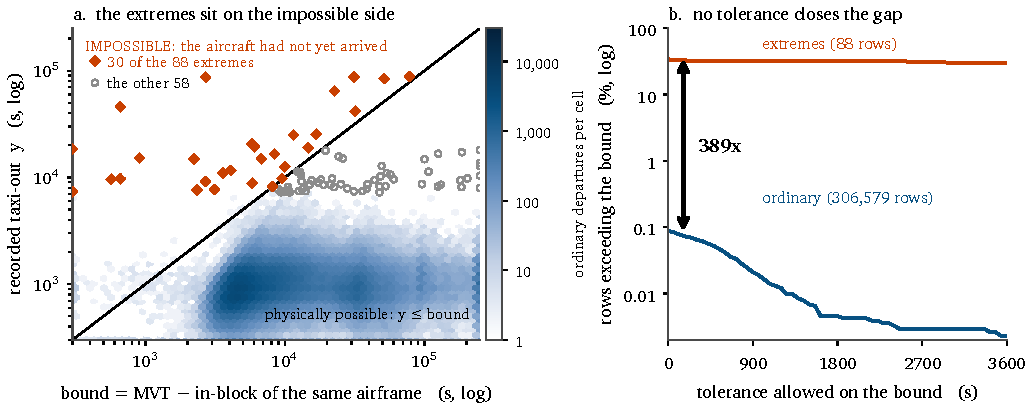
\includegraphics[width=\textwidth]{figures/physical-bound.pdf}
  \caption{Recorded taxi-out against the bound from the same airframe's previous in-block (a), and the share above it by tolerance (b). Ordinary departures sit below it; a third of the extremes sit above it, and no tolerance out to an hour closes the gap.}
  \label{fig:1}
\end{figure}

The 0.097\% on ordinary rows tests the chain rather than the label. A wrong registration match would produce violations at random, on ordinary rows as readily as on extremes; there are almost none on ordinary rows, so the chain is essentially exact and the violations among the extremes are in the label. Section~\ref{sec:4.4} shows how such a value is written: when an airport's system has no actual off-block it writes the scheduled time into the off-block field, and a scheduled time can predate the aircraft's arrival. The identity key decides whether the constraint can be measured at all. A stand-based guess at the airframe, the aircraft that last occupied the same stand, violates the same bound on 99.45\% of the rows where the bound is tight enough to matter, where the true registration gives 0.097\%. \ref{sec:C.2} recovers identity from the movement database itself.

\subsection{Trajectories falsify the record}\label{sec:4.2}

The adsb.lol archive~\cite{adsblol} publishes, for every day, the position reports that a volunteer network of ADS-B receivers heard from every aircraft. If they heard an aircraft in the air during its recorded taxi, the record is wrong. Six labelled extremes fall on the days of the first traces examined for this question, all at Fiumicino. Five match a trace and resolve to an airframe through \texttt{icao24}, the aircraft's 24-bit transponder address, a key the operational extract does not contain, and four of the five answer the question the same way (Table~\ref{tab:3}):

\begin{table}[htbp!]
  \centering
  \small
  \setlength{\tabcolsep}{1.9pt}\renewcommand{\arraystretch}{1.15}
  \caption{Four extremes whose aircraft were airborne during their recorded taxi (Fiumicino, dated by take-off), with two ADS-B samples of each airframe from inside that taxi: the time, the distance from the airport and the altitude.}
  \label{tab:3}
  \begin{tabular*}{\linewidth}{@{\extracolsep{\fill}}llrllllrr}
  \toprule
  \textbf{Flight} & \textbf{Date} & \textbf{\texttt{y} (s)} & \textbf{Recorded off-block} & \textbf{Take-off} & \textbf{Airframe} & \textbf{Seen at} & \textbf{Distance (km)} & \textbf{Altitude (m)} \\
  \midrule
  ARGG1141 & 2025-06-11 & 19,851 & 17:15:04 & 22:45:55 & LV-GHQ & 20:04 & 29.9 & 3,840 \\
   &  &  &  &  &  & 20:14 & 11.4 & 320 \\
  \addlinespace
  RYRYR7ER & 2025-09-15 & 9,121 & 20:34:59 & 23:07:00 & EI-DCX & 21:46 & 28.9 & 2,316 \\
   &  &  &  &  &  & 21:55 & 11.8 & 320 \\
  \addlinespace
  WMT7TL & 2025-09-15 & 15,967 & 07:34:56 & 12:01:03 & 9H-WDZ & 09:44 & 33.7 & 2,164 \\
   &  &  &  &  &  & 09:52 & 7.3 & 305 \\
  \addlinespace
  WZZZ2062 & 2025-09-15 & 41,700 & 19:25:00 & 07:00:00 & 9H-WAF & 05:27 & 27.5 & 968 \\
   &  &  &  &  &  & 05:30 & 11.4 & 312 \\
  \bottomrule
  \end{tabular*}
\end{table}

Every one of the four is a descent profile into the departure airport. In the first row the record has the aircraft off its stand at 17:15:04; at 20:04 it is 29.9 km out at 3,840 m, and at 20:14 11.4 km out at 320 m, still descending. None of the four had landed when its record says it left the stand: the last airborne sample shown comes 3.0, 1.3, 2.3 and 10.1 h after the recorded off-block, and none of the four has any sample within 30 km of the field in the six hours before its recorded off-block. The fifth landed before its claimed off-block and has no sample during its claimed taxi, so it neither confirms nor refutes. All six have \texttt{BLOCK\_TIME} equal to \texttt{SCHED\_TIME} within five seconds, with \texttt{LOBT}, \texttt{AOBT\_3} and \texttt{AIRCRAFT\_TYPE} null: the recorded off-block is the schedule, and the flight-plan fields are empty.

Whether a receiver can see the apron is a property of the airport, and it sets what ADS-B can do there. At Fiumicino the first ADS-B contact of an ordinary departure is the take-off roll (three ordinary departures first appear at -7, +13 and -648 s relative to take-off), so the apron is not observed there and only the airborne question can be answered; Amsterdam and Zurich acquire an aircraft within 0 to 8 minutes of its recorded off-block. Event feeds derived from ADS-B tracks follow the same line of sight: runway-entry events exist at all ten airports (Amsterdam 8,650 and Frankfurt 8,662 flights per 10 days), while parking-position exit events exist only at Zurich and Frankfurt. So on the extreme rows ADS-B can falsify a recorded off-block and cannot recover one, because no off-block event occurred to be observed. On genuine rows it can, and Section~\ref{sec:5.2} builds on that.

\subsection{How the records are written}\label{sec:4.3}

A timestamp's resolution identifies the system that wrote it: a schedule lands on exact minutes and mostly on five-minute marks, a clock read to the second rarely lands on either, and a clock rounded to the minute favours no five-minute mark. It can be read from the data alone (Table~\ref{tab:4}):

\begin{table}[htbp!]
  \centering
  \small
  \setlength{\tabcolsep}{5pt}\renewcommand{\arraystretch}{1.15}
  \caption{Timestamp resolution by column, labelled 2025 records.}
  \label{tab:4}
  \begin{tabular*}{\linewidth}{@{\extracolsep{\fill}}lrrl}
  \toprule
  \textbf{Column} & \textbf{Exact minute} & \textbf{Five-minute mark} & \textbf{Reading} \\
  \midrule
  \texttt{SCHED\_TIME} & 100.0\% & 100.0\% & A schedule \\
  \texttt{IOBT}, \texttt{LOBT}, \texttt{EOBT\_1} & \textasciitilde100\% & \textasciitilde95\% & Filed \\
  \texttt{ARVT\_1} & 1.7\% & 0.3\% & Machine-captured, one-second \\
  \texttt{AOBT\_3} & 97.7\% & 19.9\% & Machine, rounded to the minute \\
  \texttt{ARVT\_3} & 29.9\% & 6.0\% & Mixed: two pipelines feed one column \\
  \bottomrule
  \end{tabular*}
\end{table}

Seven of the ten airports (EDDM, EGLL, LEBL, LEMD, LFPG, LIRF, LTFM) put 8.3\% of their recorded off-block times on an exact minute, against the 1.7\% expected of a clock that writes seconds; the other three sit at 1.7 to 2.0\%. The 8.3\% is one in twelve, and the shape says why: at those seven airports 99.99\% of \texttt{BLOCK\_TIME} values fall in the twelve seconds from :54 to :05 and are flat inside them, and a stamp spread flat over twelve seconds lands on the exact minute one time in twelve. The column there carries a minute-resolution stamp plus about six seconds of jitter (Figure~\ref{fig:2}). Barcelona and Madrid write \texttt{MVT\_TIME} to the second and \texttt{BLOCK\_TIME} to the minute.

\begin{figure}[htbp!]
  \centering
  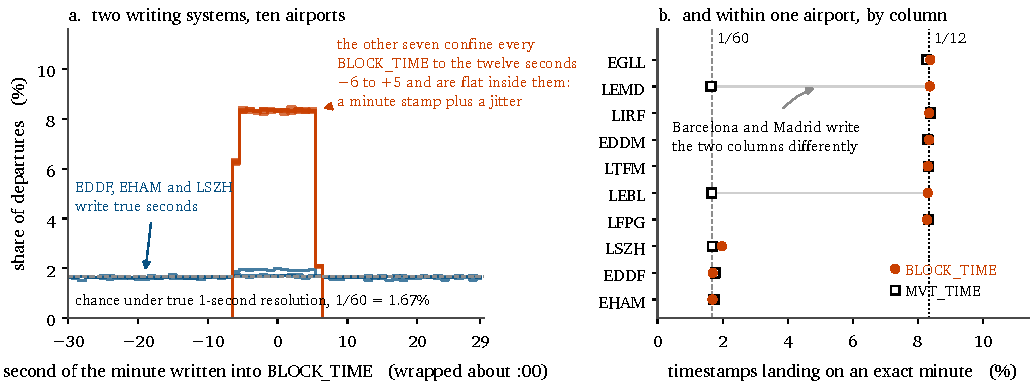
\includegraphics[width=\textwidth]{figures/clock-grid.pdf}
  \caption{Timestamp resolution separates the ten airports into two writing systems with nothing in between, and separates two columns inside one airport. The coarse group is not on a five-second grid: it writes a minute stamp with about six seconds of jitter.}
  \label{fig:2}
\end{figure}

Resolution identifies the writer and says nothing about what the writer knew. The rows that land on an exact minute without copying any other column, between 3,412 and 18,133 per airport, have the same median target as the other ordinary rows to three significant figures (836 against 838 s, 779 against 775, 1,320 against 1,321, 960 against 965), with the same or lower extreme rate. Every per-row resolution flag lands at a lift of 0.1 to 0.3 on extremes, so a row carrying one is less likely to be extreme, and none predicts an exact schedule match (\texttt{BLOCK\_TIME\ ==\ SCHED\_TIME}) above a lift of 1.2. Nullity is all-or-nothing: of the eight observable timestamps, a row has either none null or six, never a number in between.

The network's off-block, \texttt{AOBT\_3}, is the obvious off-block to lean on, and at most airports it is a computation rather than an observation. If the network set it as the take-off time minus a standard taxi time for the stand and runway, then \texttt{naive\ =\ MVT\ -\ AOBT\_3} would be nearly constant within an (airport, stand, runway) group while the airport's own record of the same flights varied. Among genuine departures, Table~\ref{tab:5} gives the share whose \texttt{naive} lies within 60 s of its group median, beside the spread of \texttt{naive} and of \texttt{y} within those groups:

\begin{table}[htbp!]
  \centering
  \small
  \setlength{\tabcolsep}{3pt}\renewcommand{\arraystretch}{1.15}
  \caption{The network's implied taxi time against the airport's record, genuine 2025 departures, within (airport, stand, runway) groups: the share of \texttt{naive} within 60 s of its group median, and the within-group standard deviations.}
  \label{tab:5}
  \begin{tabular*}{\linewidth}{@{\extracolsep{\fill}}lrrrrrrrrrr}
  \toprule
  \textbf{In a group} & \textbf{LEBL} & \textbf{LEMD} & \textbf{LSZH} & \textbf{EDDM} & \textbf{LTFM} & \textbf{EDDF} & \textbf{LFPG} & \textbf{LIRF} & \textbf{EHAM} & \textbf{EGLL} \\
  \midrule
  \texttt{naive} within 60 s of median & 97.5\% & 97.4\% & 93.2\% & 84.4\% & 71.9\% & 64.4\% & 51.9\% & 49.2\% & 31.1\% & 17.5\% \\
  SD of \texttt{naive} (s) & 110 & 101 & 102 & 166 & 188 & 122 & 276 & 136 & 298 & 395 \\
  SD of \texttt{y} (s) & 222 & 213 & 227 & 247 & 321 & 229 & 307 & 344 & 228 & 335 \\
  \bottomrule
  \end{tabular*}
\end{table}

At the six airports on the left of the table, Barcelona to Frankfurt, the airport's record varies on the same rows where the network's taxi time does not, so the network's ``actual'' off-block is, for most flights, a lookup applied to the take-off time. At Istanbul the lookup can be read off directly: on 90.3\% of 2025 departures (88.8\% in 2026) the take-off minus the network's off-block lies within 10 s of a whole number of minutes set by the runway direction, mostly 19 or 20 on the north-flow runways (35L, 35R, 36) and 24 or 25 on the south-flow ones (16R, 17L, 17R, 18), and on those rows it correlates with the recorded taxi at 0.194. There the strongest feature a model of this target has, \texttt{naive}, carries the stand-and-runway standard and nothing about the individual flight. At Amsterdam and Heathrow it varies more than the airport's own record and is measured. The airports write no default taxi time into their own records; the network writes one into its record of them. Where both clocks are measured they still disagree by a per-airport offset (median -296 s at Istanbul, -109 s at Amsterdam, -87 s at Frankfurt) that drifts by up to three minutes between months, and airport, month, hour, stand and carrier together explain at most 19.6\% of the disagreement.

\subsection{One airport writes the schedule when it has no off-block}\label{sec:4.4}

If different airports wrote different things when they lack an off-block, a survey should find several conventions. Across the 2,085,047 labelled departures, five candidates were tested for what \texttt{BLOCK\_TIME} might be a copy of: the scheduled time, the flight-plan off-block time, the initial off-block time, a default taxi time (which would place a spike on the target), and a clock-rounded entry. A sixth, a stale record equal to the same flight's off-block on an earlier day, was tested on the ten labelled departures whose recorded off-block sits about a day before their schedule, and matched 0 of 10.

Only the schedule copy exists, and only at Fiumicino. The flight-plan and initial off-block copies track the schedule copy everywhere and add nothing. No airport has a default taxi time: the largest probability mass on any single value of the target at any airport is 0.49\%, the mode of a continuous distribution. A punctual pushback lands on its scheduled minute, so some copies arise by chance: nine of ten airports sit at the 6 to 10\% rate chance produces under a realistic off-block distribution; Fiumicino runs at 20.7\%.

Around the exact copy sits a wider habit: records that disagree with the network look punctual. Of 7,946 departures whose recorded off-block is more than 30 minutes before the network's, 65.9\% are logged within 15 minutes of schedule while the network places them a median 52 minutes late (Fiumicino 89\%, Heathrow 70\%, Amsterdam 7\%). A natural suspicion is that records are placed to stay under a reporting threshold, and the data do not support it: the recorded delays do not pile up below 15 minutes, 2 hours or 3 hours beyond what the network's own delays show, so the habit is not aimed at a punctuality or passenger-rights threshold~\cite{ec261_2004}.

Among recorded taxis longer than 45 to 50 minutes, records of this kind, whose off-block precedes the network's by 30 minutes or more, outnumber those whose long taxi the network confirms; between 60 and 90 minutes the network confirms a long taxi on 5.4\% of rows, and between 90 and 120 minutes on 1.4\%.

\textbf{A corrupted identifier.} \texttt{FLIGHT\_mvt} sometimes carries the three-letter airline designator followed by its own last \emph{k} characters, \texttt{prefix\ =\ D\ +\ D{[}-k:{]}} with k in \{1, 2, 3\}: \texttt{ITY} written \texttt{ITYTY}, \texttt{BAW} as \texttt{BAWW}, \texttt{RYR} as \texttt{RYRRYR}. The pattern spans 108 distinct designators and 2,951 rows in 2025. Without a failed join it is inert and holds no extreme. Together with a failed flight-plan join it is the sharpest cell in the dataset, 161 rows of which 95 are extreme (59.0\%), against a 0.028\% base rate, a lift of 2,107. One cause produces both symptoms. A corrupted identifier cannot match a flight plan, which produces the null callsign, and the same broken record is the one whose off-block was never captured, which produces the fallback to the schedule. Every extreme in the cell has \texttt{BLOCK\_TIME} within seconds of \texttt{SCHED\_TIME}. It is a defect in an upstream pipeline rather than a property of the airport.

Rows carrying the fallback have the entire flight-plan record null, a failed join. A failed join has two possible causes, and they imply opposite things. Either the flight exists in the flight table and this movement failed to link to it, in which case the airport had the data, or the flight was never there, in which case the airport had nothing and wrote the schedule. Flight-number rarity separates the two. A number operating once a month is a charter or an extra section, for which the airport holds no stable record, while a daily service is properly in the system. Rarity is counted as appearances per 30 days within the period covered, since a raw count drifts about 6x between a 365-day and a 62-day pool. On Fiumicino's 2025 departures in the failed-join cell (Table~\ref{tab:6}):

\begin{table}[htbp!]
  \centering
  \small
  \setlength{\tabcolsep}{5pt}\renewcommand{\arraystretch}{1.15}
  \caption{Schedule-copy rate by flight-number rarity, Fiumicino, 2025, failed flight-plan join.}
  \label{tab:6}
  \begin{tabular*}{\linewidth}{@{\extracolsep{\fill}}lrr}
  \toprule
  \textbf{Flight-number appearances per 30 days} & \textbf{Rows} & \textbf{Copy rate} \\
  \midrule
  {[}0.00, 0.25) & 110 & 91.82\% \\
  {[}0.25, 0.60) & 34 & 88.24\% \\
  {[}0.60, 1.50) & 39 & 87.18\% \\
  {[}1.50, 4.00) & 57 & 80.70\% \\
  {[}4.00, 12.00) & 124 & 62.90\% \\
  {[}12.00, inf) & 233 & 38.63\% \\
  \bottomrule
  \end{tabular*}
\end{table}

The copy rate falls steadily as the flight number becomes more frequent. The signal is within carriers rather than a proxy for the operator: inside the four carriers whose own schedule-copy rates are indistinguishable from a coin flip, the rarest flight numbers still copy at 89.47\% against 37.24\% for the most frequent.

\subsection{Two further mechanisms}\label{sec:4.5}

\textbf{A one-day date error from joining two clocks.} Twelve 2025 departures at Fiumicino carry an off-block with the correct clock time on the previous calendar day, so their target is 86,400 s plus an ordinary taxi. Measured on all 1,488 Fiumicino departures of 2025 with no flight plan attached (\texttt{LOBT} null), in Europe/Rome local time:

\begin{itemize}
\item
  every one of the 12 rollovers has \texttt{localdate(BLOCK)\ ==\ localdate(SCHED)} and \texttt{localdate(MVT)\ ==\ localdate(SCHED)\ +\ 1};
\item
  none of the 1,320 rows that do not cross the local date rolled over;
\item
  crossing rows with \texttt{MVT\ -\ SCHED\ \textgreater{}=\ 20,000\ s} are 36 schedule copies, 11 rollovers and 0 ordinary rows;
\item
  non-crossing rows with \texttt{MVT\ -\ SCHED\ \textgreater{}=\ 30,000} are 8 of 8 schedule copies and 0 rollovers.
\end{itemize}

\begin{figure}[htbp!]
  \centering
  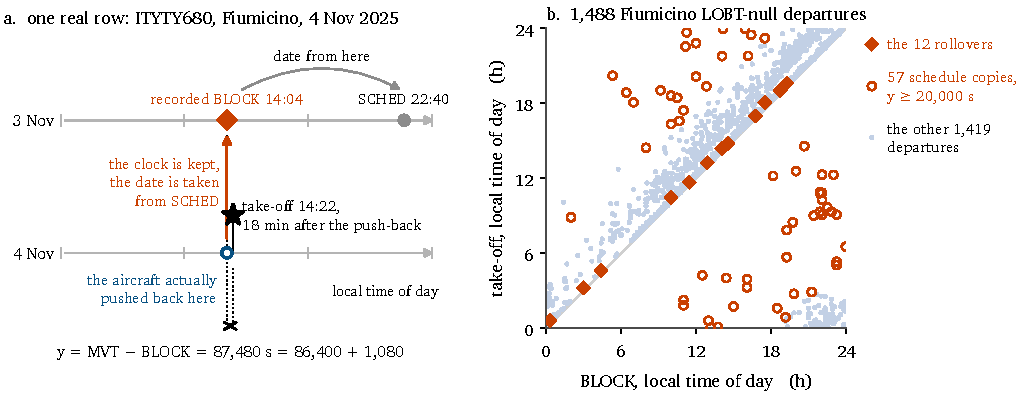
\includegraphics[width=\textwidth]{figures/date-error.pdf}
  \caption{One rollover (a) and Fiumicino's 1,488 plan-less departures by local time of off-block and take-off (b). The record keeps the real push-back's clock time and the schedule's date, so the twelve rollovers look ordinary on the clock and are wrong only by a day.}
  \label{fig:3}
\end{figure}

The corrupted \texttt{BLOCK\_TIME} is the schedule's local date joined to the actual off-block's local time of day: a date resolved against the wrong reference, which is why the clock survives intact while the date does not (Figure~\ref{fig:3}). The construction gives a necessary condition. The defect can appear only when the take-off crosses the local date relative to the schedule, because otherwise the two dates coincide and the join does nothing. Two further rows in the labelled year sit at the same magnitude by different constructions, one at Zurich and one at Paris; both look ordinary on every observable, and the necessary condition is Fiumicino's alone.

\textbf{The return-to-stand double push.} Two departure records can exist for one flight, with take-offs seconds apart, from different stands:

\begin{footnotesize}
\begin{verbatim}
LFPG AFR1192  take-off 09:54:53  BLOCK 07:51:57  stand J37  callsign AFR1192  y = 7376
LFPG AFR1192  take-off 09:54:59  BLOCK 09:23:01  stand J04  callsign NaN      y = 1918
\end{verbatim}
\end{footnotesize}

The aircraft pushed, was sent back, pushed again from another stand and departed; both pushes were written as movements, and the first carries a two-hour taxi. Detected as the same flight number at the same airport with two departures within 900 s, the pattern covers 232 of 2,085,047 rows, 29 of them extreme (12.5\%), a lift of 446. It is a different mechanism from the schedule fallback, and its long taxi is physically real: only 3.4\% of these extremes have \texttt{y} equal to the schedule deviation, against 74.0\% of all extremes. The pair separates on an observable: the member whose flight-plan join succeeded is 21.4\% extreme and its twin 4.2\%.

Paris shows the same event within a single record. On all 30 of its 2025 extremes with a flight plan, the recorded off-block lies more than an hour before the network's, and on 29 the network's implies an ordinary taxi of at most 30 minutes: the airport keeps the first pushback and the network the last. Another aircraft in-blocked at the same stand between the recorded off-block and the take-off on 40.5\% of Paris's extremes, against 7.0\% of its ordinary departures, so on those rows the stand had been vacated at the recorded time.

\subsection{A carrier's feed fails, and the arrivals show it}\label{sec:4.6}

At Fiumicino the schedule copy behaves as a property of the carrier, which we read as a property of its ground handler: when a handler does not feed the airport's off-block system, the carrier's departures are written at their scheduled time, and the failure often reaches the arrivals the same handler serves, whose in-block is then written at the scheduled arrival time. The second symptom is the useful one: arrivals keep their labels in the scored months, so each carrier's arrival feed in January and July 2026 can be read from the file even though its departures are blanked. Here a record, arrival or departure, is copied when its block time lies within 60 s of the scheduled time; an arrival is counted only when it lands more than 600 s early, where a copied in-block is visible against the real one; and a departure is delayed when it takes off at least 900 s after its scheduled off-block.

One carrier's feed failed during the labelled year and was still down at the start of the scored one (Table~\ref{tab:7}):

\begin{table}[htbp!]
  \centering
  \small
  \setlength{\tabcolsep}{5pt}\renewcommand{\arraystretch}{1.15}
  \caption{One carrier's feed at Fiumicino (THY): schedule copies among all its departures and its early arrivals.}
  \label{tab:7}
  \begin{tabular*}{\linewidth}{@{\extracolsep{\fill}}lrr}
  \toprule
  \textbf{Period} & \textbf{Departures copied} & \textbf{Early arrivals copied} \\
  \midrule
  January to September 2025, monthly range & 4.8 to 15.8\% & 2.1 to 14.5\% \\
  October 2025 & 56.5\% of 124 & 46.4\% of 69 \\
  November 2025 & 99.2\% of 120 & 100\% of 70 \\
  December 2025 & 99.2\% of 123 & 100\% of 80 \\
  January 2026 & Blanked & \cellcolor{recordtint}100\% of 38 \\
  July 2026 & Blanked & \cellcolor{measuredtint}10.9\% of 64 \\
  \bottomrule
  \end{tabular*}
\end{table}

The two directions moved together, and the arrivals show the failure persisting in January 2026 and repaired by July. The co-movement holds beyond this carrier. Over the 53 carriers with at least six 2025 months of at least 15 early arrivals and 15 delayed departures each (584 carrier-months), each carrier's monthly arrival copy rate and its monthly delayed-departure copy rate, both taken relative to the carrier's own 2025 mean, correlate at 0.512 (weighted by the months' row counts). An outage can be timed from the arrivals as a run of at least five consecutive early arrivals of a carrier, all copied. The 2025 records hold 381 such runs over 41 carriers, and the carrier's departures inside them are copies 71.6\% of the time, against 22.2\% for the same carriers outside them.

Whether departures follow differs by carrier. Of the 36 carriers with at least ten departures inside runs in 2025, 25 follow, with 62 to 100\% of those departures copied (at least half, by our definition), and 11 do not, at 7 to 48\%, suggesting that their arrival and departure records reach the airport by different routes. The pattern is Fiumicino's alone. At the nine other airports no carrier with 30 or more delayed departures has half or more of them copied, against 16 at Fiumicino, and their early-arrival copy rates stay between 0.1 and 5.5\% in both years. The labels of a scored month thus show each carrier's arrival-feed state in that month, and, for carriers whose departures follow, the likely state of their blanked departures. Section~\ref{sec:5.3} states the two rules the final model builds on this, and Section~\ref{sec:6.3} what they paid.

\subsection{The flight-plan join is a record too}\label{sec:4.7}

The extract attaches a departure to its Network Manager flight plan only when the airport's recorded off-block lies within an hour of the plan's last filed off-block, \texttt{LOBT}: over the 2,062,577 departures of 2025 that carry a plan, \texttt{BLOCK\ -\ LOBT} spans exactly -3,606 to +3,606 s, while \texttt{MVT\ -\ LOBT} reaches 87,001 s. Whether a departure carries a plan is therefore itself a record of its hidden off-block, and it is visible in the scored months, where the off-block is blanked: a plan present means the label lies within 3,606 s of \texttt{MVT\ -\ LOBT}. Where the plan is missing at Fiumicino, the same flight's plan can sometimes be recovered from its arrival record at the destination, when the destination is one of the ten airports: for 106 of the 216 such 2025 departures bound for the ten (of 1,488 without a plan in all), and for 36 in 2026. On flights that carry both, the arrival's \texttt{LOBT} equals the departure's on 99.88\%. The join rule then decides the record in two cases (Table~\ref{tab:8}).

\begin{table}[htbp!]
  \centering
  \small
  \setlength{\tabcolsep}{5pt}\renewcommand{\arraystretch}{1.15}
  \caption{Fiumicino departures without a plan whose plan is recovered from the destination, 2025, by take-off time against the recovered \texttt{LOBT}.}
  \label{tab:8}
  \begin{tabular*}{\linewidth}{@{\extracolsep{\fill}}lrrl}
  \toprule
  \textbf{Take-off against \texttt{LOBT}} & \textbf{Rows} & \textbf{Copies} & \textbf{What the record must be} \\
  \midrule
  More than 3,606 s later & 76 & 0 & Real: a copy would have joined \\
  Within 3,606 s & 30 & 21 & An off-block more than 3,606 s before \texttt{LOBT} \\
  \bottomrule
  \end{tabular*}
\end{table}

In the first case the plan was not updated for the delay: on 69 of the 76 it still sat within the hour of the schedule, so a schedule copy would have joined, and the record did not. All 76 records are real, and the network's off-block for the same flight places them within a median 124 s. In the second case an off-block comes before its take-off, which is within the hour of the plan, so one that failed to join can only lie more than an hour before the plan: \texttt{MVT\ -\ LOBT\ +\ 3,606} is a floor under the label, and no 2025 row at Fiumicino breaks it. Where \texttt{ms} clears that floor, so that a copy is possible, 21 of the 23 rows are copies. Outside Fiumicino the first case is copy-free too, 749 rows at the nine other airports and none a copy, but the model already places those rows and the network's off-block places them worse. The floor fails there at five airports, on 4 of 6 such departures at Amsterdam and 9 of 11 at Barcelona, because a missing plan there is mostly a failed identifier match rather than the time window; Istanbul's 20 hold. Istanbul's missing plans have a different cause: 76.0\% of its 2025 departures without a plan fly to Ercan in Northern Cyprus, and none of its 2,772 departures to Ercan carries one.

Among a different 76, the Fiumicino departures of 2025 without a plan and with a schedule deviation under 30 minutes, a fourth record class appears beside the real taxi, the schedule copy and the date error: the off-block recorded one UTC offset early, as if a local time had been converted to UTC twice, so that \texttt{y} is a taxi plus the offset, 3,600 s in January and 7,200 s in July. It covers 20 of the 76, and 17 of the 21 departures of six carriers. No arrival at Fiumicino shows it in either year, so its state in the scored months cannot be read from the arrivals.

These consequences of the join, and the classifier of Section~\ref{sec:5.3}, were found by a separate AI agent session given only the challenge's files and our model's predictions. We re-derived the join rule and both recovered-plan cases with independent code before any submission used them; the classifier we checked for any use of a scored departure's label, and used as written.

\section{Models}\label{sec:5}

The model has three parts; the reading of Section~\ref{sec:4} decides which acts on a row. A \textbf{base model} predicts every row, with a mixture that can replace its regression by a timestamp copied from the record. A \textbf{trajectory stage} corrects it where an open sensor saw a real pushback. \textbf{Rules read from the record} act where the airport wrote something other than a pushback, mostly at Fiumicino.

Figure~\ref{fig:4} draws the parts from real rows, one band each: the record of one departure at Amsterdam, whose pushback ADS-B saw seven seconds before the off-block the airport recorded; the base model's blend weights and its mixture on one Fiumicino row; the trajectory stage's ground samples and its effect by airport; THY's records at Fiumicino, copied or not; and the competition model's score on the 2026 set after each part.

\begin{figure}[htbp!]
  \centering
  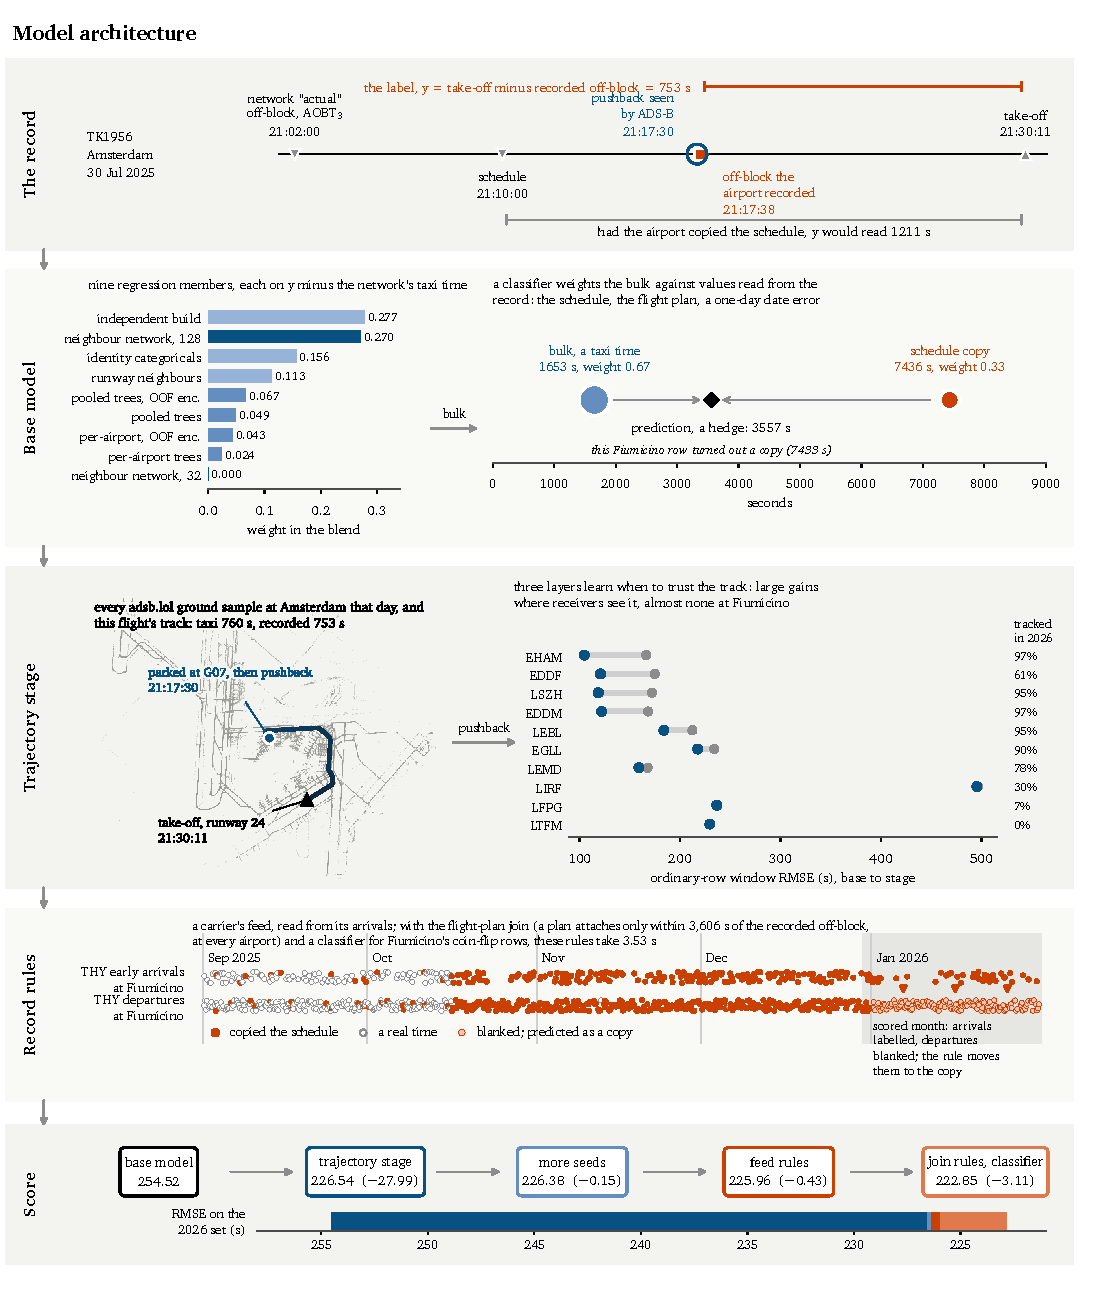
\includegraphics[width=\textwidth]{figures/model-architecture.pdf}
  \caption{Model architecture, drawn from real rows: one departure's record, the base model, the trajectory stage, the rules read from the record, and the competition model's score on the 2026 set after each part (its trajectory stage includes the refitted weight; Table~\ref{tab:summary} lists the two steps separately).}
  \label{fig:4}
\end{figure}

\subsection{The base model}\label{sec:5.1}

The base model has two steps. The first is the blend of nine regression members, each trained to predict an ordinary taxi time; its output is the \textbf{bulk}, the prediction for a row whose record is a taxi. The second is a five-branch mixture that can replace the bulk with a timestamp copied from another column of the same record. The mixture exists because on the extreme rows the target is not a taxi time at all, and the correct answer is a different column. The base model reads no trajectory data.

\textbf{Target construction.} The regression members do not predict \texttt{y} directly. Each predicts \texttt{y\ -\ naive}, how far the taxi departs from the one the network's off-block implies, with \texttt{naive\ =\ MVT\ -\ AOBT\_3} where \texttt{AOBT\_3} exists (98.9\% of departures), falling back to the airport-hour median of \texttt{naive} and then to its global median. The choice matters: on an earlier validation split of the labelled year, a network predicting \texttt{y} directly scored 409.32 s, and the same network on the residual target 406.27 s.

\textbf{Training population.} Every regression member trains on ordinary rows only, \texttt{y\ \textless{}\ 7,200\ s}. The extremes are left to the mixture, because a record-keeping failure and a long taxi are different quantities, and one estimator fitted to both is worse at the first.

\textbf{Features.} The tree members read 71 columns built from the record's timestamps, traffic counts, aggregates of \texttt{naive}, target encodings and published air traffic flow management (ATFM) statistics; \ref{sec:B} lists them, with every member's settings and the blend weights.

\textbf{Neighbour networks.} Two members are neural networks that read, through attention, what no tabular member sees: the nearest other movements at the same airport (\ref{sec:B} gives the architecture).

What a network may read about a neighbour is fixed by what the evaluation blanks. A neighbouring \emph{arrival's} taxi-in is labelled everywhere, including in the 2026 file, and is read; a neighbouring \emph{departure's} taxi-out is blanked and is never read. The observed-taxi input and its mask are therefore identically zero on every departure neighbour, so that ``no departure label is read'' can be checked in the input cache. The tabular congestion features (departure and arrival counts, runway gap, pushback count) are hand-chosen summaries of exactly this set, which is why an attention model over it decorrelates from them.

\textbf{Mixture.} A gradient-boosted classifier on a feature subset, calibrated by isotonic regression so that its probabilities match observed rates, gives each row a probability vector $P$ over five branches, and the prediction mixes the branch values:

\begin{align}
  V &= [\, \mathit{bulk},\ \mathit{ms},\ \mathrm{MVT}-\mathrm{LOBT},\ \mathrm{clip}(86{,}400+\mathit{bulk}),\ \mathit{bulk} \,]
     \label{eq:mixture} \\
  \pi &= P^{0.90}, \text{ renormalised; weights below 0.10 on branches 1 to 4 are set to zero} \nonumber \\
      &\phantom{={}} \text{and their mass returned to branch 0} \nonumber \\
  \hat{y} &= \mathrm{clip}( \mathrm{round}( \textstyle\sum \pi V ),\ 60,\ 2 \times 10^{5} ) \nonumber
\end{align}

Branch 0 is the regression, branch 1 the schedule copy, branch 2 the flight-plan copy and branch 3 the one-day date error. Branch 4 returns the regression as well, duplicating branch 0, so the mixture has four distinct values. Branches 1 to 3 are the \textbf{copy branches}: each copies a timestamp from the record instead of predicting a taxi. A row with some probability on a copy branch gets a prediction between the regression and the copy, a \textbf{hedge}. A hedge is wrong on every row, since the record holds one value or the other, and it costs error on the rows that turn out ordinary; it is what a squared-error loss asks for when the copy is uncertain. The two constants in the mixture, the exponent 0.90 and the floor 0.10, sit at a swept optimum: moving the exponent costs 0.0761 s at 0.80 and 0.3669 s at 1.00, and moving the floor costs 3.9179 s at 0.05 and 0.3881 s at 0.15.

The floor bounds every result here that would reach the output through the mixture. A weight below 0.10 is set to zero, so a signal that moves a branch's probability by less than ten points cannot reach the output at all. Several effects measured in Section~\ref{sec:4}, among them the lift of 1.30 that a schedule copy on the aircraft's previous leg gives (\ref{sec:C.1}), are real and sit under that floor.

\textbf{Two versions, and the two models.} The base model exists in two versions, because its two scoring sets need different training data. The \textbf{validation version} is scored on the window: its members are trained on the ten months of 2025 outside the window, and its mixture is the learned one above. The \textbf{submitted version} is scored on the 2026 set: its members are trained on all of 2025, and the mixture's branches are applied through a hand-built chain of rules instead of the classifier, each replacing the prediction on a chosen cell and each fitted on labelled data, including the carrier-level cells of \ref{sec:E.4} and the date branch of Section~\ref{sec:4.5}. On the 2026 set the two agree within 60 s on 99.46\% of rows; the submitted chain moves 251 rows more than 600 s off the bulk, the learned mixture 175.

The two versions give the two models this paper reports. The competition model is the submitted version with everything this work added to it on the 2026 set, including the constants described next. The final model applies the validation version's learned mixture to the scored rows, adds the two cells of the hand-built chain whose evidence is labelled, and carries no value fitted to a score on the 2026 set; Section~\ref{sec:7} gives its construction and its scores. The stage and the rules of the next two subsections were first built and measured on the competition model, as Section~\ref{sec:6} reports them.

\textbf{Constants fitted to returned scores.} Some constants in the submitted version were fitted to scores returned by the 2026 set. They are present in the competition model and absent from the final model; the repository's \texttt{REPRODUCE.md} (section 9) lists them and their measured effect, and Section~\ref{sec:6.3} measures the model without them.

\subsection{The trajectory stage}\label{sec:5.2}

The trajectory stage corrects the base model where the record is a real pushback and a sensor observed it (Section~\ref{sec:4.2}): raw ADS-B surface tracks from the open adsb.lol archive~\cite{adsblol}, with substantial coverage at seven of the ten airports and some at two more. It lowers the RMSE on the 2026 set by 27.99 s with its weight refitted (27.71 s as first submitted), 4.6428e9 of squared error (Table~\ref{tab:15}).

All 365 days of 2025 and the 62 scored days of 2026 in the archive were streamed and reduced to what the features need, take-offs, landings and ground samples at the ten airports, with no raw trace kept.

\textbf{The match.} A departure is matched to a trace by callsign and a take-off within 300 s. Many take-offs carry an empty callsign, which arrives in the trace only after lift-off, so a second pass matches on time alone: same airport, take-off within 60 s, and each candidate the other's only one. Run blind on 17,474 departures whose callsign match was known, the second pass is right on 10,499 of the 10,522 pairs it makes, 99.78\%, and makes a pair for 60.2\% of them. Time-matched rows are safe to apply the stage to and harmful to train it on: included in training, they cut the gain on callsign-matched window rows from 1.6977e9 to 1.4360e9 of squared error, while themselves gaining 4.3e7.

\textbf{The pushback.} The detector looks at the airframe's ground samples at the airport in the 3 h before its take-off, keeps those after the last gap longer than 900 s, and needs at least three. Two cases follow. If the aircraft is parked when first seen (ground speed at most 1 kt and less than 10 m of displacement over its first three samples), the pushback is the first sample that has moved more than 15 m or exceeds 2 kt: a \textbf{dwell} detection, named for the wait it observes before the push. Otherwise the transponder came on during the push or later, and the pushback is the first sighting: a \textbf{first-seen} detection. For a first-seen departure, the last place the airframe was seen parked in the previous 18 hours, usually the end of its inbound flight, measures how much was missed. It exists for 91.3\% of departures with a pushback; the distance from it to the first departure sighting is a median 106 m, a transponder switched on at the stand, and 1,217 m at the 90th percentile, a late sighting.

Over all of 2025, the detected pushback lands within 60 s of the airport's recorded off-block on 30.7\% of the 1,075,086 genuine departures that have one, against 23.7\% for the network's clock on the same rows; dwell detections land within 60 s on 64.1\%, and first-seen ones on 26.4\%, a median 230 s late. By airport it is closer to the record than the network's clock at Amsterdam, Munich, Zurich and Barcelona and further from it at Madrid, Fiumicino, Heathrow and Paris (Table~\ref{tab:17}). A raw detection is therefore a strong but biased measurement at some airports and a late one at others, which is why the stage learns when to trust it rather than copying it.

\textbf{Coverage.} A row with a detected pushback is \textbf{covered}. Coverage belongs to the receiver network rather than to the method, and the network changed between the years. Table~\ref{tab:9} gives the share of departures with a detected pushback, in percent:

\begin{table}[htbp!]
  \centering
  \small
  \setlength{\tabcolsep}{5pt}\renewcommand{\arraystretch}{1.15}
  \caption{Departures with a detected pushback, by airport and period (\%).}
  \label{tab:9}
  \begin{tabular*}{\linewidth}{@{\extracolsep{\fill}}lrrrrrrrrrr}
  \toprule
   & \textbf{EDDF} & \textbf{EDDM} & \textbf{EGLL} & \textbf{EHAM} & \textbf{LEBL} & \textbf{LEMD} & \textbf{LFPG} & \textbf{LIRF} & \textbf{LSZH} & \textbf{LTFM} \\
  \midrule
  Window, Jan + Jul 2025 & 89.1 & 61.8 & 38.0 & 98.0 & 93.9 & 15.3 & 2.1 & 53.1 & 93.1 & 0.0 \\
  2026 set, Jan + Jul 2026 & 60.6 & 96.9 & 89.8 & 96.9 & 94.7 & 78.0 & 7.3 & 29.8 & 95.0 & 0.0 \\
  \bottomrule
  \end{tabular*}
\end{table}

A pushback is detected for 60.9\% of the 2026 departures, against 50.3\% of the window's. Istanbul has no surface receiver in either year and Paris almost none; Fiumicino had none in January 2025 and has none in July 2026. The gap is the receivers and not the matcher: of 87,088 departures of the 2026 set without a pushback, at the nine airports with any coverage, only 685 have an unclaimed take-off within 60 s whose airframe was seen on the ground in the hour before it.

\textbf{Where the stage acts.} The stage sits on top of the base model and never overrides its mixture. It changes only covered rows whose base prediction is not a schedule copy (it differs from the copy by more than 60 s), and it leaves alone the rows the mixture hedges toward a copy. The window says why. Among the covered window rows where the base predicts above 3,600 s there are 328; 74.1\% of them are ordinary by count, but only 5.9\% by the squared distance between the two hypotheses. Replacing the base prediction with the bulk there, which is what trusting the track would mean, costs 3.47e10 of squared error, because on the day-scale records that carry the mass the aircraft's track shows an ordinary departure and the record does not.

\textbf{Inputs.} They describe the aircraft's movement: the detected taxi and its difference from the base prediction, the dwell before the push, distances at first sighting and at the push, sample count and largest gap, stationary time, first speed, path length, a stop in the last fifteen minutes, the take-off offset and the parked-position quantities above, 25 in all.

\textbf{Three layers.} The first corrects the base model's error on covered rows; the second retrains the base model's tree members with the trajectory inputs over the whole year and replaces the bulk on covered rows; the third corrects the second's error. The covered-row prediction is a weighted average of the first layer and the other two.

\textbf{Layer 1: a residual stage on the base model.} Gradient-boosted trees on the base model's error, trained on January and July 2025 (cross-fitted on the window). The gain is the sensor's: on the covered rows the base model's own inputs, given the same stage, remove nothing (-3.38e7 on a 24-day run), and the detected taxi blended linearly per airport removes a twentieth of what the learned stage does (Table~\ref{tab:10}):

\begin{table}[htbp!]
  \centering
  \small
  \setlength{\tabcolsep}{5pt}\renewcommand{\arraystretch}{1.15}
  \caption{Layer 1 on the window, on the base model: squared error removed on covered window rows, January and July cross-fitted, by the learned stage and by a linear blend of the sensor.}
  \label{tab:10}
  \begin{tabular*}{\linewidth}{@{\extracolsep{\fill}}lrr}
  \toprule
  \textbf{Learner} & \textbf{SSE removed} & \textbf{SE} \\
  \midrule
  Trees on trajectory and base inputs & +1.6496e9 & 6.54e7 \\
  Per-airport linear blend of the detected taxi & +8.22e7 & 1.56e7 \\
  \bottomrule
  \end{tabular*}
\end{table}

The stage that ships averages four learners in equal parts: LightGBM~\cite{ke2017lightgbm}, XGBoost~\cite{chen2016xgboost}, CatBoost~\cite{prokhorenkova2018catboost} and an MLP, with the XGBoost settings frozen from one automated search~\cite{wang2021flaml}.

\textbf{Layer 2: full-year bulk members.} The base model's pooled and per-airport tree recipes with the trajectory features added, trained on all twelve months of 2025. On the window, trained on the other ten months, the pooled member scores 206.735 s on ordinary rows against 226.020 for its base-model counterpart, and the per-airport member 211.775 against 231.395. They must replace the base bulk and the layer-1 stage on the rows they cover rather than sit beneath them: a stage fitted to the base's residual already carries the signal, so stacking the two counts it twice, and the stacked construction's estimated gain was -1.8587e9 of squared error. Where no pushback exists, their blend weight refits to zero.

\textbf{Layer 3: a full-year stage.} Equal halves of LightGBM and XGBoost on out-of-fold residuals of the full-year bulk (the error of a layer-2 model that did not train on the row), with folds by month: five two-month folds inside the ten non-window months for the window's predictions, six over all twelve for the 2026 set's. It is trained on 1,132,994 covered, callsign-matched ordinary rows and applied where the full-year bulk is under 3,600 s.

\textbf{The weight between the layers.} On covered rows the submitted prediction moves from the layer-1 model toward the layer-2-and-3 model by a weight of 0.837, fitted on the window's covered rows outside Fiumicino and stable between the months (0.834 fitted on January, 0.840 on July). Fiumicino keeps layer 1 alone: fitted per airport, its weight on that move is 0.370, against 0.59 to 0.95 everywhere else. The weight was first fitted with Fiumicino in, at 0.662: Fiumicino had no coverage in January 2025, so its rows sit in July alone, and they pulled the July fit down to 0.589.

\subsection{Seeds, and rules read from the record}\label{sec:5.3}

After the stage and its refitted weight, the competition model adds the nine changes of Table~\ref{tab:11}; the final model carries all of them except the extra seeds, and applies the day-scale bands of Section~\ref{sec:7} after them. Each was submitted with two numbers written down beforehand: its predicted score, and its \textbf{kill line}, the score at or above which it would count as a failure. The join bound and the first recovered-plan case went together; the others went one at a time. None carries a weight fitted to a score on the 2026 set; every rate is counted on labelled 2025 rows, the arrivals of the scored months, which keep their labels, show each carrier's feed state, and no rule reads the label of a scored departure.

\begin{table}[htbp!]
  \centering
  \small
  \setlength{\tabcolsep}{5pt}\renewcommand{\arraystretch}{1.15}
  \caption{The changes after the trajectory stage: the rows each moves on the 2026 set, and its evidence.}
  \label{tab:11}
  \begin{tabularx}{\linewidth}{>{\raggedright\arraybackslash\hsize=0.9\hsize}Xr>{\raggedright\arraybackslash\hsize=1.25\hsize}X>{\raggedright\arraybackslash\hsize=0.85\hsize}X}
  \toprule
  \textbf{Change} & \textbf{Rows} & \textbf{2025 evidence} & \textbf{Read from 2026} \\
  \midrule
  More seeds in three members & Every row & The seeds' spread on the scored rows & No label \\
  THY's feed & 118 & 241 of 243 THY departures copied in November and December & THY's early arrivals, 38 of 38 copied in January \\
  Outage spans by carrier class & 81 & 25 of 36 carriers' departures followed their arrivals & Outage spans in the arrivals \\
  Join bound & 29 & \texttt{BLOCK\ -\ LOBT} within 3,606 s on all 2,062,577 departures with a plan &  \\
  Recovered plans, first case & 22 & 76 of 76 real &  \\
  Coin-flip classifier & 271 & 1,248 departures, 46.0\% copies & The carrier's arrival copy rate \\
  Recovered plans, second case & 14 & 21 of 23 copies where \texttt{ms} allows; no row below the floor &  \\
  Local-time class & 27 & 20 of 76 &  \\
  Day-scale floor & 6 & 45 rows: 36 copies, 9 date errors, none real &  \\
  \bottomrule
  \end{tabularx}
\end{table}

\textbf{More seeds.} Three members average more seeds than when first submitted: 18 instead of 8 for the 128-neighbour network, 10 instead of 2 for the independently built member (\ref{sec:B}), and 10 instead of 3 for the full-year pooled member of layer 2. The scored rows' own spread between seeds measures the seed variance without labels: the expected gain was 2.693e7 of squared error, and the 2026 set paid 2.3724e7. The extra seeds were trained for the 2026 set only, so the window has no counterpart.

\textbf{A carrier whose feed is down.} The 2025 failure of Section~\ref{sec:4.6} fixes a rule for THY at Fiumicino. In a scored month in which THY's early arrivals are at least 90\% copied, on at least ten of them, each THY departure whose schedule deviation lies inside the failure's 2025 range (its 1st to 99th percentile, 62 to 5,695 s) is predicted as \texttt{0.992\ *\ clip(ms)\ +\ 0.008\ *\ bulk}, almost the schedule copy, where 0.992 is the failure's departure copy rate (241 of 243 in November and December 2025), \texttt{clip} the submissions' {[}60, 200,000{]} s and \texttt{bulk} the base model's. January 2026, its arrivals 38 of 38 copied, opens the rule; July, at 10.9\%, does not, and neither month of the window does.

\textbf{Outage spans by carrier class.} The outage runs of Section~\ref{sec:4.6} extend the same reading to every carrier. An outage span is a run of at least five consecutive early arrivals of one carrier, all copied, from the first to the last. The rule selects a 2026 Fiumicino departure inside a 2026 span of its own carrier, with a schedule deviation inside the 1st to 99th percentile of the 2025 departures inside spans. Its prediction \texttt{v} already sits between the bulk and the copy, at an implied copy weight of \texttt{(v\ -\ bulk)\ /\ (clip(ms)\ -\ bulk)}; where that weight is below a target \texttt{w}, the prediction moves to \texttt{w\ *\ clip(ms)\ +\ (1\ -\ w)\ *\ bulk}. For a carrier that followed in 2025, \texttt{w} is its own copy rate inside its 2025 spans; for a carrier with no 2025 span, \texttt{w} is 0.731, the rate expected of a carrier of unknown class: 25 of 36 carriers followed, copying 96.1\% inside their spans, and the rest copied 20.9\%. A carrier that did not follow, or that had fewer than ten departures inside its 2025 spans, is left alone. In 2026 the range of schedule deviation is -2 to 11,776 s.

\textbf{The join bound.} Section~\ref{sec:4.7} found every 2025 label with a plan within 3,606 s of \texttt{MVT\ -\ LOBT}. The rule applies that bound: every prediction for a departure that carries a plan is clipped onto \texttt{{[}MVT\ -\ LOBT\ -\ 3,606,\ MVT\ -\ LOBT\ +\ 3,606{]}}, at every airport.

\textbf{Recovered plans at Fiumicino.} The two cases of Table~\ref{tab:8} become two rules for a Fiumicino departure without a plan whose plan is recovered from the destination. If it took off more than 3,606 s after the recovered \texttt{LOBT}, the record is real, and the prediction is the take-off minus the \texttt{AOBT\_3} of the arrival record. If it took off within 3,606 s, the off-block lies more than 3,606 s before \texttt{LOBT}: the prediction is raised to \texttt{MVT\ -\ LOBT\ +\ 3,606} where it sits below, and where \texttt{ms} exceeds that floor it moves to \texttt{0.913\ *\ clip(ms)\ +\ 0.087\ *\ prediction}, 0.913 being the 2025 copy rate of the case (21 of 23).

\textbf{Fiumicino's coin flip.} The departures without a plan delayed one to four hours are the rows the file leaves nearest a coin flip: 1,248 in 2025, 46.0\% of them schedule copies. Where their plan cannot be recovered, a gradient-boosted classifier of the copy probability \texttt{P}, from the agent session of Section~\ref{sec:4.7} and built from the provided data only, re-weights them. It reads \texttt{ms}, the local hour and weekday, whether the take-off crossed the local date, the carrier's copy and delay-filing habits (its copy rate combined with how often its copies and its real records lack a plan), the day's count of such departures and its delayed fraction, the carrier-day counts of delayed and plan-less departures, the carrier's same-day delay filing on departures that do carry a plan, its arrival copy rate that day and that month, a malformed-callsign flag, and stand, runway and destination. The prediction becomes \texttt{0.5\ *\ (taxi\ +\ P\ *\ (ms\ -\ taxi))\ +\ 0.5\ *\ prediction}, with \texttt{taxi} the 2025 median real taxi for the local three-hour period; the weight 0.5 is the midpoint, not fitted to a score.

\textbf{Fiumicino's local-time records.} Departures without a plan and with \texttt{ms} under 1,800 s, whose plan cannot be recovered, may hold the fourth record class of Section~\ref{sec:4.7}, an off-block one UTC offset early. They take a mixture of an ordinary taxi of 1,000 s, that taxi plus the offset, and the schedule copy, \texttt{p\_real\ *\ 1,000\ +\ p\_tz\ *\ (1,000\ +\ offset)\ +\ p\_copy\ *\ clip(ms)}, with the class rates counted on 2025: for the six carriers of Section~\ref{sec:4.7}, 0.810 local-time and 0.095 each real and copy; for the rest, 0.436 real, 0.055 local-time and 0.509 copy.

\textbf{Day-scale delays without a plan.} A Fiumicino departure without a plan delayed 30,000 to 86,000 s was never a real record in 2025: of 45, 36 were schedule copies and 9 date errors, and no date error fell below 46,800 s. Below that the prediction becomes \texttt{clip(ms)}; above it, \texttt{ms} is a floor. Identifiers corrupted by a repeated airline designator (Section~\ref{sec:4.4}) are left out: an earlier commitment of that cell to the schedule copy lost on the 2026 set, so its 2025 rate is not evidence for the scored months, and one of those rows would have carried 82\% of the move. A second session of the same agent found the rule; we checked it before submission. The final model does not use that score: its day-scale bands apply the 2025 rates to those identifiers too.

\section{Results}\label{sec:6}

\subsection{Baselines and accuracy by airport}\label{sec:6.1}

Four predictors are compared on the window (Table~\ref{tab:12}). The first is \texttt{naive}, the taxi time implied by the network's off-block (\texttt{MVT\ -\ AOBT\_3}, with the fallbacks of Section~\ref{sec:5.1}). The second is each airport's median 2025 taxi-out, taken from the ten months outside the window. The other two are the base model and the competition model.

On the window the competition model is replayed so that no rule learns from the window's own labels. The stage keeps its refitted weight. The outage-span rule learns everything from the ten other months (the eleven carriers the submitted base model already commits to the copy left out, \ref{sec:D}). The join bound, the first recovered-plan case and the day-scale floor learn nothing and apply as they are. The classifier, the second case's copy rate and the local-time class rates come from 2025 without the row's own month. The extra seeds have no window counterpart, and the THY rule opens in neither window month. All predictions are clipped to {[}60, 200,000{]} s as the submissions are.

\begin{table}[htbp!]
  \centering
  \small
  \setlength{\tabcolsep}{5pt}\renewcommand{\arraystretch}{1.15}
  \caption{Baselines and models on the window.}
  \label{tab:12}
  \begin{tabular*}{\linewidth}{@{\extracolsep{\fill}}lrrrr}
  \toprule
  \textbf{Window RMSE (s)} & \textbf{\texttt{naive}} & \textbf{Airport median} & \textbf{Base model} & \textbf{Competition model} \\
  \midrule
  All rows & 642.400 & 665.980 & 309.603 & 289.620 \\
  Ordinary rows & 409.110 & 420.944 & 237.367 & 213.233 \\
  \bottomrule
  \end{tabular*}
\end{table}

On the 2026 set the base model scores 254.5228 and the competition model 222.8507. On the window, the competition model's improvement over the base is 19.983 s {[}14.668, 26.486{]} on all rows and 24.134 s {[}20.789, 28.181{]} on ordinary rows, with 95\% intervals from a bootstrap that resamples the window's 62 days whole. The final model has no window column here: on the window its base differs from the competition model's only in the month offsets (\ref{sec:D}), but the chain's cells and the day-scale bands it adds are not replayed there; its scores are in Section~\ref{sec:7}.

By airport, on ordinary window rows (Table~\ref{tab:13}):

\begin{table}[htbp!]
  \centering
  \small
  \setlength{\tabcolsep}{5pt}\renewcommand{\arraystretch}{1.15}
  \caption{Ordinary-row RMSE on the window, by airport.}
  \label{tab:13}
  \begin{tabular*}{\linewidth}{@{\extracolsep{\fill}}lrrrrr}
  \toprule
  \textbf{Airport} & \textbf{Rows} & \textbf{\texttt{naive}} & \textbf{Airport median} & \textbf{Base model} & \textbf{Competition model} \\
  \midrule
  EDDF & 36,830 & 259.8 & 366.8 & 175.0 & 120.9 \\
  EDDM & 27,091 & 391.2 & 355.2 & 168.4 & 122.1 \\
  EGLL & 40,190 & 477.5 & 475.7 & 234.1 & 217.8 \\
  EHAM & 40,947 & 348.1 & 371.4 & 166.5 & 104.0 \\
  LEBL & 28,985 & 323.7 & 347.0 & 212.4 & 183.9 \\
  LEMD & 35,328 & 273.0 & 312.9 & 167.8 & 159.1 \\
  LFPG & 39,580 & 369.3 & 467.9 & 237.3 & 236.6 \\
  LIRF & 26,415 & 655.6 & 665.4 & 496.5 & 456.2 \\
  LSZH & 22,283 & 273.8 & 338.7 & 172.2 & 118.8 \\
  LTFM & 46,538 & 523.5 & 414.8 & 229.8 & 229.8 \\
  \bottomrule
  \end{tabular*}
\end{table}

The network's own off-block is a poor predictor on its own, worse than a constant per airport at three of the ten airports (Munich, Heathrow and Istanbul); what makes it useful is the models' residual construction around it. The ordinary-row figures for the two models include the cost of the mixture's hedge (Section~\ref{sec:5.1}): on an ordinary row, any move toward the copy is error. At Fiumicino that cost is large, and neither model comes close to its accuracy elsewhere. The trajectory stage improves the airports its receivers see (Frankfurt, Munich, Amsterdam and Zurich most) and leaves Istanbul, which it cannot see, unchanged.

\subsection{Where the error sits}\label{sec:6.2}

\begin{figure}[htbp!]
  \centering
  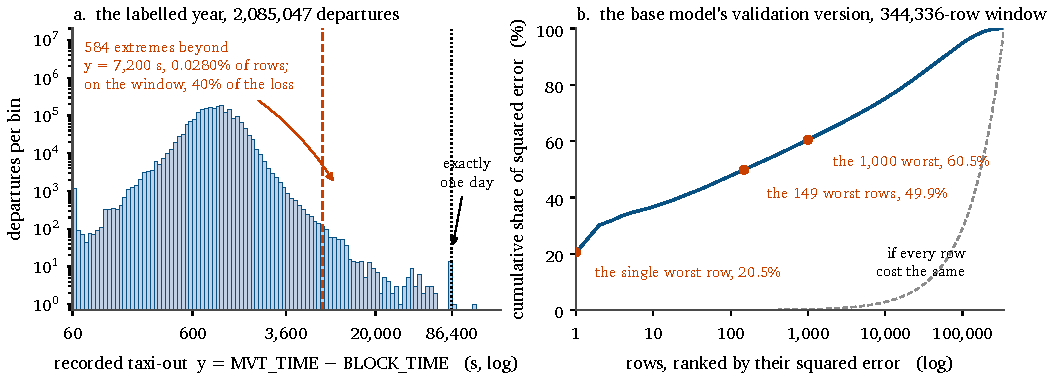
\includegraphics[width=\textwidth]{figures/loss-concentration.pdf}
  \caption{Recorded taxi-out in the labelled year (a) and cumulative squared error by ranked row on the window (b). 584 of 2,085,047 labelled departures exceed 7,200 s, and under the base model's validation version the single worst row carries a fifth of the 344,336-row window's squared error.}
  \label{fig:5}
\end{figure}

An \textbf{oracle} here is the base model with perfect information of one kind substituted on one set of rows, for example the true value of every extreme; the RMSE it reaches says what that information alone would buy. Measured on the validation version of the base model before its final blend (309.603 s after it, Table~\ref{tab:12}), over the window's 344,336 rows and 149 extremes, with every oracle changing only its own rows (Table~\ref{tab:14}):

\begin{table}[htbp!]
  \centering
  \small
  \setlength{\tabcolsep}{5pt}\renewcommand{\arraystretch}{1.15}
  \caption{Oracle decomposition on the window, validation version of the base model before its final blend.}
  \label{tab:14}
  \begin{tabular*}{\linewidth}{@{\extracolsep{\fill}}lrr}
  \toprule
  \textbf{Window} & \textbf{RMSE (s)} & \textbf{Gain (s)} \\
  \midrule
  Validation version of the base model & 313.8931 &  \\
  Perfect extreme magnitude (extreme rows exact) & 242.9062 & 70.99 \\
  Perfect extreme detection (extremes set to their conditional mean) & 292.8497 & 21.04 \\
  Perfect bulk (ordinary rows exact) & 198.8101 & 115.08 \\
  \bottomrule
  \end{tabular*}
\end{table}

Extremes are 0.0433\% of rows and carry 40.12\% of the squared error (Figure~\ref{fig:5}), and the model lands within 600 s of 18 of the 149. Knowing their exact values is worth 70.99 s; knowing which rows they are, without their values, 21.04 s, about 30\% of that. The schedule-copy channel points the same way from the other side: perfect copy detection is worth +24.04 and perfect copy magnitude +24.21 RMSE-equivalent seconds, so once a row is known to be a schedule copy the schedule gives its value for free, and detection is 99.3\% of that channel.

These proportions describe the window: its two largest rows, day-scale records at one airport that no observable flags, carry 30.2\% of the window's squared error. The 2026 set appears to contain no such row (Section~\ref{sec:3}), so there the ordinary rows carry most of the error and the perfect-bulk line is the larger gain too.

\subsection{What each change bought}\label{sec:6.3}

Table~\ref{tab:summary} gives the score on the 2026 set after each part of the competition model, and of the same design without its fitted constants. The trajectory stage carries most of the gain and the rules read from the record most of the rest. \ref{sec:D} lists every change with its estimate on the window, what acting directly on each mechanism of Section~\ref{sec:4} is worth, and the rules' effects in detail.

\begin{table}[htbp!]
  \centering
  \small
  \setlength{\tabcolsep}{5pt}\renewcommand{\arraystretch}{1.15}
  \caption{The competition model, part by part, and the same design without the constants fitted to the 2026 set, to the final model.}
  \label{tab:summary}
  \begin{tabular*}{\linewidth}{@{\extracolsep{\fill}}lr}
  \toprule
  \textbf{Model} & \textbf{RMSE on the 2026 set (s)} \\
  \midrule
  Base model, no trajectory data & 254.5228 \\
  \quad + trajectory stage & 226.8129 \\
  \quad + refitted weight & 226.5352 \\
  \quad + more seeds & 226.3833 \\
  \quad + carriers' feed rules & 225.9576 \\
  \quad + join rules, classifier, local-time class, day-scale floor (competition) & \textbf{222.8507} \\
  \midrule
  Clean base, no fitted constants & 292.0485 \\
  \quad + trajectory stage & 268.1373 \\
  \quad + the same rules & 247.7412 \\
  \quad + two labelled chain cells, refitted weight, day-scale bands; rebuilt on four months (final) & \textbf{233.7464} \\
  \bottomrule
  \end{tabular*}
\end{table}

The lower half of the table rebuilds the design without the constants fitted to returned scores (Section~\ref{sec:5.1}), with the learned mixture for the tail, as on the window, and month offsets estimated on labelled data; the final model is built on that clean base (Section~\ref{sec:7}). The gap between the two bases holds both the fitted constants and the hand-built chain's Fiumicino rules (\ref{sec:D}).

\subsection{What one RMSE resolves}\label{sec:6.4}

One row from the base model's window residuals shows the scale. An ordinary-looking departure at Paris (carrier EJU, stand C03) has a schedule deviation of 1,740 s, a recorded \texttt{y} of 84,240 s and a prediction of 759 s. Its squared error alone is 6.969e9, equal to 31.2\% of the submitted base model's squared error on the 2026 set. One such row in the 2026 set would move a model's score by about 38 s of RMSE, where the first trajectory layer, the largest single change in Table~\ref{tab:15}, moved 2.7319e9 of squared error, 0.39 of one such row.

On heavy-tailed operational targets a single-number RMSE therefore resolves far less in the tail than its reported precision suggests, because whether a tail record separates two models depends on whether the scored draw happens to contain one. A trimmed or winsorised companion metric, or a bootstrap interval over scored rows, would separate method from draw. The 2026 set appears to contain none (Section~\ref{sec:3}), so the reported differences are differences in method and in data.
\section{The final phase}\label{sec:7}

At the close, the organisers added February and June 2026 to the scored months and asked for one final file covering all four, to be ranked without feedback on January and July, on February and June, and on the four together. The new extract holds 670,790 departures: the 344,841 of January and July, the same movements as before, and 325,949 in February and June. Every arrival in the four months keeps its taxi-in time. The January and July rows differ from the earlier extract in one respect: each movement's take-off time moves by up to 12 s. On arrivals, where both timestamps are visible, the recorded block time moves by the opposite amount (the two shifts correlate at $-0.990$ over 344,693 arrivals), so a departure's label moves by about twice its take-off shift.

The final model is the file uploaded for the final ranking. It carries no constant fitted to a returned score, and its composition was fixed before its one score. It is retrained once on the twelve 2025 files, at the members' original seed counts (Section~\ref{sec:5.3}), and predicts the four months together with one code path, \texttt{scripts/final/run\_final.sh}. Every value on that path is counted on labelled 2025 rows or read from the scored months' labelled arrivals:
\begin{itemize}
\item the mixture's weights on its copy branches, which decide how far a row moves from the regression toward a copied timestamp, come from the learned mixture of Section~\ref{sec:5.1} applied to the scored rows, as on the window, and not from the competition model's hand-built chain;
\item a month offset is a constant added to every prediction of one month, the model's mean residual on labelled ordinary rows of that month. For January ($-10.656$\,s) and July ($-0.528$\,s) it is the bulk's own on the window, with the blend weights refitted while each month is allowed its own intercept; February ($+3.800$\,s) and June ($+2.727$\,s) are not in the window, so theirs come from a single tree model cross-fitted over the twelve months;
\item two cells of the hand-built chain, the two whose evidence is labelled, enter at their 2025 rates: a block of stands at Fiumicino whose 28 labelled rows hold no schedule copy, and eleven carriers whose 1,688 labelled 2025 rows with a schedule deviation above 600 s are schedule copies at 99.11\%;
\item every step of the trajectory stage keeps the variant it used on the window; four steps had chosen theirs by a comparison on the scored rows, which on four months would weigh different rows, so the choice is fixed to the one made before. The stage's blend weight of Section~\ref{sec:5.2} refits outside Fiumicino to 0.837 on this base (0.826 fitted on January, 0.847 on July);
\item the rules of Section~\ref{sec:5.3} apply as stated there, without the extra seeds;
\item at Fiumicino, a departure without a flight plan and delayed 20,000\,s or more against its schedule is predicted as a mixture of a schedule copy, a date error and the prediction so far, weighted by the 2025 counts of Table~\ref{tab:final_bands} for its band, the corrupted identifiers of Section~\ref{sec:4.4} included.
\end{itemize}
Two traces of the fitted values remain on this path; the blend weights' trace that \ref{sec:D} finds in the earlier rebuilds is removed here by refitting them. The trajectory stage's XGBoost settings were searched against the residual of a base that carried the fitted month offsets, and the coin-flip classifier of Section~\ref{sec:5.3} trains on the competition model's predictions for the window rows. The repository's \texttt{FINAL.md} lists every value with its source.

\begin{table}[htbp!]
  \centering
  \small
  \caption{Fiumicino departures without a flight plan and a schedule deviation of at least 20,000\,s, labelled 2025. A date error is possible only where the departure crosses the local date; the one non-crossing row above 50,000\,s takes the pooled non-crossing rate.}
  \label{tab:final_bands}
  \begin{tabular*}{\linewidth}{@{\extracolsep{\fill}}lrrrr}
  \toprule
  \textbf{Band} & \textbf{Rows} & \textbf{Schedule copy} & \textbf{Date error} & \textbf{Ordinary} \\
  \midrule
  20,000 to 50,000\,s & 50 & 48 & 0 & 2 \\
  50,000\,s or more, crossing the local date & 19 & 8 & 11 & 0 \\
  50,000\,s or more, not crossing & 1 & 1 & 0 & 0 \\
  \bottomrule
  \end{tabular*}
\end{table}

The competition model's file ships beside it, to compare the two models. It takes January and July from the competition model, with the 509 of its predictions that are a function of the take-off time (417 schedule copies, 63 take-off minus \texttt{LOBT}, 29 at a flight-plan bound) recomputed from the new extract's take-off times, since those moved, and February and June from the final model.

The last three submissions before the upload were each written down with an expected score and a decision rule beforehand (Table~\ref{tab:final_scores}). The first resubmitted, unchanged, the model of \ref{sec:D} rebuilt without the fitted constants and carrying the trajectory stage and the rules (Mixture+T+R); it returned its earlier score to four decimals, so the scored labels had not moved. The second replaced the weight the learned mixture puts on the schedule copy with the competition model's classifier, recalibrated on labelled data. On the window this change had no detectable effect ($-5.64\times10^{7}$ of squared error, day-clustered standard error $2.66\times10^{8}$), and the rule fixed beforehand adopted it only if it gained more than one window standard error. It lost $9.15\times10^{7}$, and the final model keeps the learned mixture. The third scored the final model's own January and July rows. Its expected score priced two changes from their 2025 rates, the day-scale bands and the eleven carriers' cell, and nothing else; the day-scale rows carry most of the interval's width (Section~\ref{sec:8}).

\begin{table}[htbp!]
  \centering
  \small
  \caption{January and July 2026 on the leaderboard. February and June have no feedback.}
  \label{tab:final_scores}
  \begin{tabular*}{\linewidth}{@{\extracolsep{\fill}}lrr}
  \toprule
  \textbf{Submission} & \textbf{Expected} & \textbf{Scored} \\
  \midrule
  Competition model & & 222.8507 \\
  Mixture+T+R, resubmitted unchanged & 247.7412 & 247.7412 \\
  Mixture+T+R, copy weight from the competition classifier & 247.41 [244.34, 250.45] & 248.2763 \\
  Final model, January and July rows & 239.25 [232.60, 245.73] & 233.7464 \\
  \bottomrule
  \end{tabular*}
\end{table}

On January and July the final model scores 233.7464, the score that measures the method, and the competition model, whose score includes values fitted to those months, 222.8507. The 10.90 s between them holds the constants of Section~\ref{sec:5.1}, the extra seeds, the hand-built chain's remaining cells and the retraining, which these scores do not separate. On February and June the two files carry the same predictions, made without feedback.

\section{Limitations}\label{sec:8}

\textbf{The 2026 set was reused.} This work submitted to it 90 times. Repeated scoring on one set lets selection overfit it~\cite{blum2015ladder,dwork2015reusable}: a change kept because it scored well on these rows is partly fitted to them, so the scores reported on the 2026 set are optimistic by an amount the set itself cannot measure. The window intervals of Section~\ref{sec:6.1} are the uncertainty this paper can state. Every change of Section~\ref{sec:6.3} had its score predicted before submission, but a prediction does not remove selection: the decision to keep a change was made on its score on the 2026 set. The final model's composition was fixed before its one score on the 2026 set, and February and June were predicted without feedback (Section~\ref{sec:7}).

\textbf{Day-scale records at ordinary schedule deviations cannot be found from the observables.} Across the 2,085,047 labelled departures, 76 rows carry a day-scale recorded taxi time. For 71 of them the schedule deviation is itself extreme, so an observable flags them. The other five have an ordinary schedule deviation and a day-scale target, and every observable on them looks normal. All five share one marker, a null flight-plan off-block time, which occurs on 1.078\% of rows, a lift of 92.8; it is a single condition, since the flight-plan, initial and network off-block timestamps are null on exactly the same rows, with 0 disagreements in 27,760 null rows across both years. The marker is unusable. Its cell holds 22,470 rows for 5 targets, and predicting a day-scale value on a row that is in fact ordinary costs $(86{,}400 - \mathit{taxi})^2$, the same order as the gain on a true one, so the cell would have to be 50.9\% day-scale records to break even; five in 22,470 leaves it 2,288 times short.

The learned mixture already carries the branch these rows need, the one that adds a day to the regression (branch 3 of Section~\ref{sec:5.1}). Seven rows of the window require that branch and carry 85.5\% of all extreme squared error there; the branch's weight on them averages 0.161, and its maximum anywhere in the 344,336 rows is 0.277. Committing those seven to the branch would remove 1.078e10 of the window's squared error, and committing every row whose weight passes a threshold loses at every threshold, including one at 71.4\% precision, because almost all of that sits in two rows whose weight is 0.00, which no threshold on the weight can select. A model of this target is therefore exposed to a draw it cannot see coming.

\textbf{The sensor's reach.} 39.1\% of the departures of the 2026 set have no detected pushback, all of Istanbul and nearly all of Paris among them, and a better matcher would reach at most 685 of the 87,088 at the airports with any coverage. If every departure first seen already moving, outside Fiumicino, reached the accuracy of those seen at the push, the window would gain about 2.2e8 of squared error. The learners are saturated on these inputs: a member built without the base model, a linear one and a monotone one each lose when blended in (-3.4791e8, -5.8353e7 and -2.6465e7), and a second tree family for the full-year bulk correlates with the first at 0.9952. The pushback's agreement with the recorded off-block varies by airport (Table~\ref{tab:17}), and the stage's value was measured over all 62 window days together. The archive behind the stage is a volunteer receiver network, whose coverage changed between the two years and can change again.

\textbf{Reproduction is exact only from archived components.} The neural members re-draw on every run, and multithreaded LightGBM training can move some tree members slightly, so the exact rebuilds read archived predictions; rebuilt from raw data, the base model differs from its submitted file by 9.8 s RMS (Reproducibility statement).

\textbf{Scope.} One year of labelled data at ten airports, each with its own recording systems. The mechanisms of Section~\ref{sec:4} are properties of those systems, observed here, and another airport's database may write its failures differently. The measurement lessons of \ref{sec:E} were established on this dataset; they are stated in a form that does not depend on its airports, but whether they hold elsewhere is untested.

\section{Conclusion}\label{sec:9}

The taxi-out times in this dataset are records, and a system without an off-block writes something else: at Fiumicino the scheduled time, sometimes with the schedule's date joined to the real pushback's clock time. At six of the ten airports the network's own actual off-block is, for most flights, computed rather than observed. The final model measures the pushback where one was recorded and, where the file allows, reconstructs the record where none was; with no constant fitted to scores on the 2026 set, it gains from both (Sections~\ref{sec:6.3} and~\ref{sec:7}).

For performance monitoring the findings have a direct reading. Where the reports behind the European indicator of additional taxi-out time~\cite{eurocontrol_atxot2023} are the records studied here, a schedule copy at Fiumicino enters the indicator as a long taxi that did not happen, and at the airports where the network's off-block appears to be a stand-and-runway lookup, a taxi time computed from it measures the lookup rather than the flight.

The remedy for the largest errors lies upstream of any model. A model can reconstruct a record only as far as the file shows how it was written, and Section~\ref{sec:8} shows records for which it shows nothing. Three changes where the records are written would remove the failure modes this paper had to reconstruct: writing a missing off-block as missing rather than as the schedule, which removes the schedule copy; recording whether each time was captured or filled in, which makes the fallback visible; and resolving dates against the event's own clock, which removes the date error.

What the records and the sensor cannot show bounds the model (Section~\ref{sec:8}): a day-scale record at an ordinary schedule deviation looks normal on every observable, so a single RMSE separates method from draw only when the scored draw holds none (Section~\ref{sec:6.4}), and the stage learns nothing where no receiver hears the apron, as at Istanbul and nearly all of Paris. What we learned about measuring gains on such a target is stated in \ref{sec:E}.


\section*{Acknowledgement}
The EUROCONTROL Performance Review Unit and the OpenSky Network organised the challenge and answered questions in public, and participants discussed open data sources in its public channel. We thank SoK, whose post there that their team used adsb.lol prompted us to pull that archive in full; the trajectory stage of Section~\ref{sec:5.2} grew from it. The analysis used the OPDI flight list and the adsb.lol archive; it contains information from adsb.lol, made available under the ODbL 1.0.

\section*{Open data statement}
The challenge data are distributed by the organisers of the PRC Data Challenge 2026 to registered teams and are not
redistributed with this work. The external data the models use are open: the OPDI flight list, the PRU air traffic flow
management statistics, and the adsb.lol archive of ADS-B traces, whose derived tables are not redistributed. The repository's \texttt{EXTERNAL-DATA.md} lists each source and its
licence.

\section*{Reproducibility statement}
The code is released under the GNU GPL v3 at \url{https://github.com/arquicanedo/taxi-out-as-a-record}. The repository's README gives the reproduction steps; \texttt{REPRODUCE.md} documents every model, with a byte-identical rebuild of each from archived components and a from-scratch path, and pins the library versions (\texttt{requirements.txt}).

Before release we re-ran every production stage of the base model from the published code in an empty environment and compared each output with the original. The tree models, the feature tables and the external-data joins reproduce exactly, and a fresh download of the OPDI flight lists is byte-identical to ours. The neural components re-draw on every run on Apple Metal, and the prediction chain amplifies one of them: it reconstructs an archived submission's mixture weights through the MLP, so a 6 s re-draw of the MLP moves the delivered model by 30 s RMS. The repository therefore archives the neural predictions the chain reads. With them the base model's submission rebuilds byte-identically; rebuilt entirely from raw data, it differs from the submitted file by 9.8 s RMS.

The trajectory stage, the competition model's later changes and the rebuilds without fitted constants each rebuild with one script that asserts the sha256 of every submission it writes: \texttt{scripts/regen\_adsb.sh}, \texttt{scripts/reproduce\_final.sh}, \texttt{scripts/regen\_clean.sh} and \texttt{scripts/v127\_build.sh}. The final model and the competition model's four-month file are built by \texttt{scripts/final/run\_final.sh}, documented in the repository's \texttt{FINAL.md}. The extra seeds of Section~\ref{sec:5.3} and the classifier's probabilities for the scored rows are archived (\texttt{artifacts/seeds/}, \texttt{artifacts/fable/}), because their training re-draws or is multithreaded; \texttt{scripts/fable\_lirf/} rebuilds the classifier from the challenge's files. For the adsb.lol data, licensed under ODbL 1.0, the release carries the scripts that rebuild the derived tables from the archive's public daily releases, their content hashes and the attribution notice. Tables rebuilt that way are equal in content to the originals, from which every submission rebuilds byte-identically.

\section*{Use of AI}
This work was done with the Claude Code agent (Anthropic) running Claude Opus 5 and 5.5, with Claude Fable 5.1 and Sonnet 5 subagents for independent review and verification; the agents wrote the code, ran the analyses and drafted this text under the author's direction and review. Over the logged sessions, 8 September to 5 October 2026 (the project's first week predates the logs), the author directed them with 979 prompts in 16.5 hours of interaction, measured from the logs with at most 75 seconds counted per reply; a language-model classifier judged 338 of the prompts (35\%) to introduce something the agents had not raised. The agents produced 13.95 million output tokens and worked 143.6 hours: 45.0 generating, 29.9 in subagents running in parallel, and 68.7 in computation on one laptop (Apple M5 Pro), 41.1 on its CPU and 27.6 on its GPU.

\printbibliography

\clearpage
\appendix

\section{Negative results}\label{sec:A}

The following were tried on this dataset and are closed, by measurement where a size is given and otherwise by argument: geometry (about 6 s ceiling), traffic and queue features (about 1.8 s), weather (+0.65\%), holidays, time-of-day, arrival taxi-in (arrivals anti-predict the departure offset at every timescale, negative at 9 of 10 airports, pooled -0.103), published airport-month mean taxi-out times as a constraint, three-component mixtures, pairwise overtaking graphs, destination-at-ETA, graph neural networks (four separate measurements), ACARS and every other external oracle that measures reality on the extreme rows (no sensor can recover what the airport wrote there), out-of-fold calibration at full strength (it wins attenuated, at $\alpha = 0.35$), per-row resolution and null-profile flags (Section~\ref{sec:4.3}), and the physical bound of Section~\ref{sec:4.1} enforced as a constraint (\ref{sec:D} gives its cost). The trajectory stage's own negatives are in \ref{sec:E.2} and Section~\ref{sec:8}.

Two families of record-keeping columns were tested for hidden information and carry none. Record ids are written in time order, Spearman(\texttt{MVT\_ID}, time) = 0.9929, and the gap between neighbouring ids carries nothing, a rank-gap lift of 0.9 to 1.0 at every cut; \texttt{FLIGHT\_ID} correlated to +-0.0001 with no tail. The two tables do not check each other either: four facts are recorded twice, by the movement table and the flight-plan table, every pair has a lift of 0.0 to 1.7 and most are protective (below one), and \texttt{ADEP\_mvt} and \texttt{ADEP\_flt} never disagree in 2,062,577 rows, so the two tables are not independently sourced on identity.

Three signals are worse or null on their own and positive as members of the final blend of the base model (\ref{sec:B}): the blend weights themselves, a runway-queue signal read through the observable off-block proxy of same-runway neighbours (inside ``traffic and queue features'' above), and airport-by-operator identity categoricals. Each had first been closed on an earlier validation set-up whose members differed from those that ship; what a member adds depends on what the blend already holds.

Stretching the predictions' tail to match the labels' loses on every variant (-6.53, -1.57 and -9.14 s of window RMSE): squared error rewards the conditional mean, and a prediction that averages over what it does not know is narrower than the labels by construction. A classifier separating schedule copies from genuine records inside the one airport cell where the two mix ranks them better than the incumbent (AUC 0.9199 against 0.777, unchanged with every window label deleted, and 0.9153 against 0.8086 on ten months it never saw) and buys nothing in squared error on those months, $z = -0.36$: the cell's loss sits on a few rows, and a better ranking of the many without better information on those few does not move it. Off-block times from derived parking-exit events in open trajectory data lag the recorded ones by about 300 s, with 16\% within 60 s; as a replacement for the label they are worse than the model, and raw surface tracks used beside the model are Section~\ref{sec:5.2}'s result. And row order in the published files carries no blanked information: rows run in take-off order within airport blocks, 0.9253 of consecutive pairs non-decreasing, against 0.5773 for the blanked off-block time.

Queue position (departures taking off from the same runway during a flight's own taxi) and ground density (aircraft on the ground per minute, summed above each airport's normal level) add nothing to the bulk: -0.06 and -0.16 RMSE-equivalent seconds across seasons, every airport within 1\%. The bulk predicts a correction to \texttt{MVT\ -\ AOBT\_3}, which already measures the wait, so what remains to predict is disagreement between two records of one pushback. Shared latent state is small: if the errors came from something every flight in an hour shares, errors within a runway-hour would agree, and a row's error agrees with its runway-hour's at 0.228 and with its day's at 0.104. Splitting the ordinary rows at 45 minutes, with a classifier routing each row to a short or a long model, would move the base model's score from 254.5 to about 219 on a one-to-one projection with perfect routing, and gains nothing with a real classifier (AUC 0.9885): at a 0.83\% base rate the value is in certainty, not ranking. The same holds for the Fiumicino cell of Section~\ref{sec:4.4} on its plan-present rows: a better copy classifier gains on the ten other months and loses on the two window months.

\section{Model details}\label{sec:B}

\textbf{Features.} The tree members read 71 columns, of which 7 are categorical and declared as such to the booster: airport, runway, market segment, wake-turbulence category, flight type, aircraft type and destination region. The rest are timestamp differences (\texttt{MVT\ -\ SCHED}, \texttt{MVT\ -\ LOBT}, \texttt{MVT\ -\ IOBT}, \texttt{MVT\ -\ EOBT}, \texttt{AOBT\ -\ EOBT}, \texttt{LOBT\ -\ IOBT}), filed and flown block times and their difference, cyclical time-of-day terms, traffic counts over 900, 1,800 and 3,600 s windows on departures, arrivals and the runway, airport-day and airport-hour aggregates of \texttt{naive}, eight smoothed target encodings on stand, runway, operator, airport and destination, eight published ATFM aggregates, and seven pairwise provenance indicators over the timestamp columns. The pooled tree member adds four airframe features from the OPDI flight list (\ref{sec:C.2}), 75 columns in all. The neighbour networks and the classifier read 49 of the 71, the subset that predated later feature additions. The window versions in Table~\ref{tab:18} below read a common 65 columns.

\textbf{Neighbour networks.} Attention weighs each of the nearest movements at the same airport by its relevance to the row being predicted. Each neighbour is encoded to 128 dimensions and passed through a 4-head self-attention across the set of neighbours, so that they can contextualise each other; a 4-head cross-attention then reads the set with the anchor row's own 384-dimensional stem as its query, and the head takes the concatenation of stem and attended context through 256 and 64 units. One network reads the nearest 32 movements and the other the nearest 128, both with the same six channels per neighbour. Their window versions average 3 seeds (Section~\ref{sec:5.3} gives the 2026 counts).

\textbf{The raw detection against the record.} Over all of 2025, 1,075,086 genuine departures have a detected pushback, 57.9\% of the 1,856,033 genuine departures of the year. Table~\ref{tab:17} measures it against the airport's recorded off-block, with the network's clock on the same rows:

\begin{table}[htbp!]
  \centering
  \small
  \setlength{\tabcolsep}{5pt}\renewcommand{\arraystretch}{1.15}
  \caption{Detected pushback minus recorded off-block, genuine 2025 departures with a pushback.}
  \label{tab:17}
  \begin{tabular*}{\linewidth}{@{\extracolsep{\fill}}lrrrrr}
  \toprule
  \textbf{Airport} & \textbf{Rows} & \textbf{Median (s)} & \textbf{Within 60 s} & \textbf{Within 300 s} & \textbf{\texttt{AOBT\_3} within 60 s} \\
  \midrule
  EHAM & 220,744 & -2 & 55.7\% & 86.8\% & 23.5\% \\
  EDDM & 124,117 & 46 & 53.0\% & 85.3\% & 25.8\% \\
  LSZH & 117,496 & 173 & 33.6\% & 59.5\% & 24.4\% \\
  LEBL & 153,475 & 244 & 30.1\% & 52.6\% & 26.7\% \\
  EDDF & 196,412 & 300 & 22.5\% & 49.1\% & 21.1\% \\
  LEMD & 130,215 & 384 & 5.7\% & 38.1\% & 26.1\% \\
  LIRF & 50,576 & 605 & 4.6\% & 18.4\% & 19.6\% \\
  EGLL & 72,795 & 550 & 2.1\% & 34.4\% & 19.1\% \\
  LFPG & 9,256 & 744 & 1.5\% & 5.7\% & 18.7\% \\
  \midrule
  All & 1,075,086 & 178 & 30.7\% & 58.5\% & 23.7\% \\
  \bottomrule
  \end{tabular*}
\end{table}

Dwell detections are 11.3\% of the total, with a median error of 28 s; first-seen ones are late because the transponder is often switched on after the push. At Frankfurt the raw detection is level with the network's clock. It is steady within an airport but not constant: month by month, the share within 60 s ranges from 46.1 to 60.4\% at Munich and from 33.4 to 64.6\% at Amsterdam, and on 2025-07-30, the day first examined, Amsterdam's figures were 67.6\% against 19.8\%, above its annual level.

\textbf{Pooled tree member.} Gradient-boosted trees~\cite{ke2017lightgbm}, learning rate 0.03, 6,000 trees, 511 leaves, feature fraction 0.7, over the 75 columns above, averaged over three seeds. A lighter configuration (learning rate 0.06, 2,000 trees, 255 leaves) was used in development only.

\textbf{Per-airport tree member.} The same estimator fitted separately per airport at 600 trees, 127 leaves and a minimum of 100 samples per leaf, the right capacity for roughly a tenth of the data each: the pooled configuration costs 0.82 to 2.17 s when applied here. An airport with fewer than 500 training rows falls back to the pooled prediction. The two capacities are set in different places in the code (\texttt{REPRODUCE.md}, section 3), and building both with one capacity is the easiest way to reproduce a different model.

\textbf{MLP.} Per-categorical embeddings of width \texttt{min(24,\ (cardinality\ +\ 1)\ /\ 2)}, concatenated with scaled numerics and their null masks, through 768, 384 and 192 units with GELU, batch normalisation and dropout 0.15, AdamW under a one-cycle schedule, 8 seeds averaged.

\textbf{Classifier.} Gradient-boosted trees on the 49-column set, learning rate 0.06, up to 400 iterations, 63 leaves, minimum 50 samples per leaf, L2 1.0, early stopping on a 10\% holdout with patience 40, 3 seeds averaged, then calibrated by isotonic regression against the training labels. Its output drives the mixture of Section~\ref{sec:5.1}.

\textbf{Blend weights.} Non-negative weights summing to one, the least-squares solution under those two constraints, fitted out of fold on the 344,187 ordinary window rows by a closed-form solve of the Karush-Kuhn-Tucker conditions. Table~\ref{tab:18} gives the blend before its final change, each window version's weight beside its own window RMSE on ordinary rows, clipped:

\begin{table}[htbp!]
  \centering
  \small
  \setlength{\tabcolsep}{5pt}\renewcommand{\arraystretch}{1.15}
  \caption{The base model's blend before its final change, window versions.}
  \label{tab:18}
  \begin{tabular*}{\linewidth}{@{\extracolsep{\fill}}lrr}
  \toprule
  \textbf{Member} & \textbf{Weight} & \textbf{Alone, clipped (s)} \\
  \midrule
  Pooled trees & 0.2230 & 232.916 \\
  Per-airport trees & 0.2030 & 236.380 \\
  Neighbour network, 32 neighbours & 0.0880 & 230.941 \\
  Neighbour network, 128 neighbours & 0.4860 & 229.463 \\
  Residual MLP & 0.0000 & 233.720 \\
  Neighbour networks together & 0.5740 &  \\
  Blend without the neighbour networks &  & 229.622 \\
  Blend with them &  & 225.732 (+3.890) \\
  \bottomrule
  \end{tabular*}
\end{table}

The neighbour networks take more than half the weight against three tabular members that were themselves the product of extensive feature work, and the 8-network residual MLP, which once held 0.4, is driven to exactly zero: it carried the same information, less well. In the submitted model the neighbour networks read 49 columns where the pooled trees read 75, and the 49 are a strict subset; the window versions in this table, however, all read one 65-column matrix, so the table alone does not show that the networks win on less information.

Blend members should not be selected on their standalone score. An earlier feature set made the MLP worse on its own (233.720 to 234.734) while making the blend better (229.622 to 229.491), a pure decorrelation effect.

\textbf{Target encodings.} A target encoding replaces a categorical level (a stand, a runway, an operator) with the mean target of the rows that carry it, smoothed toward the overall mean where the level is rare. The eight encodings are computed over the whole training year. A validation that trains on part of that year and scores the rest must recompute them from its training months only: computed over the whole year they contain the validation rows' own labels, and the leaked versions made each tree and network member look 0.58 to 0.94 s better on the window than its honest version. The window versions in Table~\ref{tab:18} are free of it, and every result reported in this paper was repeated without it.

\textbf{The final blend of the base model.} The submitted base model refits the weights against leak-free window versions of the members that ship, and adds five members. One is a gradient-boosted model on airport-by-operator, airport-by-stand and airport-by-carrier identity categoricals; another reads the observable off-block proxy of neighbouring departures on the same runway; a third was built independently from the raw files, a residual gradient-boosted model on 131 features (10 categorical) from a separate feature pipeline, with its own target encodings fitted out of fold on the training rows; the last two are the tree members retrained on out-of-fold encodings. Table~\ref{tab:19} gives the weights fitted on the whole window:

\begin{table}[htbp!]
  \centering
  \small
  \setlength{\tabcolsep}{5pt}\renewcommand{\arraystretch}{1.15}
  \caption{The final blend of the base model.}
  \label{tab:19}
  \begin{tabular*}{\linewidth}{@{\extracolsep{\fill}}lrlr}
  \toprule
  \textbf{Member} & \textbf{Weight} & \textbf{Member} & \textbf{Weight} \\
  \midrule
  Pooled trees & 0.0494 & Identity categoricals & 0.1562 \\
  Per-airport trees & 0.0240 & Runway neighbours & 0.1131 \\
  Neighbour network, 32 neighbours & 0.0000 & Independent build & 0.2770 \\
  Neighbour network, 128 neighbours & 0.2703 & Pooled trees, out-of-fold encodings & 0.0667 \\
   &  & Per-airport trees, out-of-fold encodings & 0.0431 \\
  \bottomrule
  \end{tabular*}
\end{table}

On ordinary window rows the leak-free replica of the previous blend scores 223.106 s and the final blend 220.496 s, with the weights fitted on one window month and evaluated on the other.
\section{Two further properties of the records}\label{sec:C}

\subsection{Schedule copies follow the aircraft}\label{sec:C.1}

The natural model of a recording failure is a station property: a particular handling agent at a particular airport does not feed the airport's system. That model is correct, and possibly incomplete. The failure is steady from day to day, and schedule copies recur along an aircraft's day beyond what the station and the operator explain. If recording failures are not independent across an aircraft's day, that matters for anyone putting error bars on such records, since independence is the usual default.

\textbf{Steady, not episodic.} A fallback is a record written at the schedule because no off-block was captured (Section~\ref{sec:3}). If fallbacks came from outages, one system would fail in both directions at once, and a run of fallback departures would sit inside a run of fallback arrivals. Pooled over airport-days, the correlation between the arrival-side and departure-side fallback rates is +0.6961, and fifty-eight percent of it is airport identity: demeaned within airport it is +0.2939 daily and +0.0810 at three-hour resolution, and on the tenth of days with the most arrival fallbacks (the top decile), departures fall back at no more than 1.33 times their usual rate anywhere. An outage would also produce days at 80 to 90\% departure fallback, and the highest departure rate on those days at any airport is 23.69\%. There are no airport-wide outage days. Within a month the fallback behaves as a steady property of the carrier, which is why a commitment on carrier identity transfers out of sample and estimates fitted on a validation window do not; over weeks to months a carrier's feed can still fail or recover (Section~\ref{sec:4.6}).

\textbf{Along the aircraft's day.} Take every departure whose aircraft can be chained to its own previous departure at a different airport, and split by whether that previous leg was a schedule copy (Table~\ref{tab:20}):

\begin{table}[htbp!]
  \centering
  \small
  \setlength{\tabcolsep}{5pt}\renewcommand{\arraystretch}{1.15}
  \caption{Schedule copies by the aircraft's previous leg at another airport, 2025.}
  \label{tab:20}
  \begin{tabular*}{\linewidth}{@{\extracolsep{\fill}}lrr}
  \toprule
   & \textbf{Chained departures} & \textbf{Copy rate} \\
  \midrule
  Previous leg was a copy & 25,657 & 11.763\% \\
  Previous leg was not & 252,015 & 9.035\% \\
  \midrule
  All & 277,672 & 9.287\% \\
  \bottomrule
  \end{tabular*}
\end{table}

The copy rate rises from 9.035\% to 11.763\%, a lift of 1.30 (Figure~\ref{fig:6}), and the lift holds within (airport, carrier) cells: LFPG/AFR 1.36, EDDF/LH1 1.31, EDDM/DLH 1.25, EGLL/BAW 1.23.

\begin{figure}[htbp!]
  \centering
  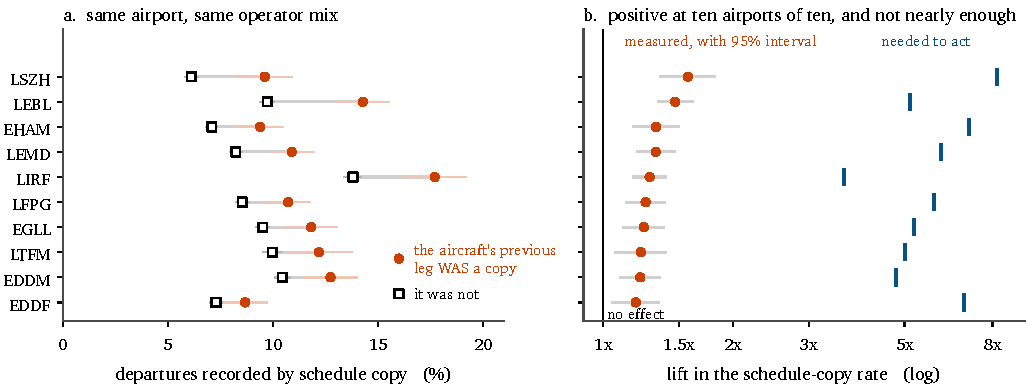
\includegraphics[width=\textwidth]{figures/airframe-carryover.pdf}
  \caption{Schedule-copy rate by airport and previous leg (a), and its lift against the lift a commitment under squared error needs (b): positive at all ten airports, and three to six times short everywhere.}
  \label{fig:6}
\end{figure}

The effect is positive at ten airports out of ten and survives conditioning on the carrier: holding both the station and the operator fixed, an aircraft whose previous departure was a schedule copy is 25 to 30\% more likely to be one again. Neither a station model nor a handler model can produce this, because both are constant within an (airport, carrier) cell. Three mechanisms are consistent with it, and the data do not separate them. The airframe may be systematically absent from the ground-handling telemetry that feeds off-block reporting, a fitment or transponder-configuration property. An aircraft already running off schedule may be handled off-process at successive stations. Or punctuality itself may persist along the day, since at nine airports most schedule copies within 60 s are punctual pushbacks rather than fallbacks (Section~\ref{sec:4.4}); that would make the carry-over a property of the operation rather than of the record.

The effect is too small to move a point prediction under squared error. A lift of 1.30 moves a 9\% base rate to 11.8\%, while committing a row to the fallback hypothesis needs roughly 50\% confidence (Section~\ref{sec:8}). Pooled, the effect delivers 2.7 of the 41.0 probability points a commitment needs, about fifteen times short; per airport the lift needed is 3.6 to 8.2, against a measured 1.19 to 1.57.

\subsection{Airframe identity is recoverable}\label{sec:C.2}

The movement database carries no tail number, no registration and no airframe key, and turnaround, stand-exclusivity and rotation analyses all need one. It still determines airframe identity exactly for a subset of flights, and approximately in general, from nothing but flight pairing and stand occupancy. The practical payoff measured here is an extreme rate of 0.0015\%, against 0.0280\% over all departures, on half the dataset.

\textbf{An exact pairing from an undocumented key.} The extract carries \texttt{FLIGHT\_ID\_mvt}, which is not documented as a pairing key. Across 4,167,797 movements it takes 3,821,595 distinct values, and 315,269 of them hold exactly one departure and one arrival. Four independent checks say that such a pair is one aircraft on one leg: the departure's and arrival's destination match on 99.483\%, their origin on 99.600\%, their aircraft type on 99.464\%, and the flight time (arrival minus departure movement time) has median 5,069 s, 1st percentile 1,895, 99th percentile 12,801, and is negative on 0.00\%. The link covers 8.2\% of flights, the share whose origin and destination both lie inside the ten-airport panel; the key is complete and the panel is not.

\textbf{Chaining by stand.} Identity extends by stand: the aircraft that in-blocks at stand X is taken to be the one that next off-blocks from X. Naively this matches 2,044,480 departures, 98.1\% of the total. Requiring the chained arrival and departure to share an aircraft type gives the chain a measurable check (Table~\ref{tab:21}):

\begin{table}[htbp!]
  \centering
  \small
  \setlength{\tabcolsep}{5pt}\renewcommand{\arraystretch}{1.15}
  \caption{Chaining by stand, 2025 departures.}
  \label{tab:21}
  \begin{tabular*}{\linewidth}{@{\extracolsep{\fill}}lrr}
  \toprule
  \textbf{Chained matches} & \textbf{Rows} & \textbf{Aircraft type agrees} \\
  \midrule
  All same-stand matches & 2,044,480 & 87.75\% (chance 6.84\%) \\
  Turnaround \textless= 14,400 s & 1,592,049 & 89.22\% \\
  \bottomrule
  \end{tabular*}
\end{table}

Type agreement is an upper bound on airframe accuracy, up to the noise in the type field itself (the exact pairing above agrees on type 99.464\% of the time), since two aircraft of the same type can swap without the check noticing. So roughly one chained match in eight is a different airframe. That error is invisible in aggregate and concentrated where it does damage: on rows whose aircraft left the stand hours before take-off, a wrong match supplies a falsely tight turnaround. Used as a physical constraint without the type filter, the bound is violated on 11 of the 13 rows it selects, so the failures fall entirely in the population the constraint exists to police. The type filter turns a useless bound into a strong one (Table~\ref{tab:22}):

\begin{table}[htbp!]
  \centering
  \small
  \setlength{\tabcolsep}{5pt}\renewcommand{\arraystretch}{1.15}
  \caption{Anomaly rate and validity of the physical bound for short turnarounds, 2025 departures.}
  \label{tab:22}
  \begin{tabular*}{\linewidth}{@{\extracolsep{\fill}}lrrr}
  \toprule
  \textbf{Turnaround \textless= 7,200 s} & \textbf{Rows} & \textbf{P(extreme)} & \textbf{Bound holds} \\
  \midrule
  Any chain & 1,197,732 & 0.0259\% & 83.07\% \\
  Type agrees & 1,037,037 & 0.0015\% & 95.18\% \\
  All departures (base) &  & 0.0280\% &  \\
  \bottomrule
  \end{tabular*}
\end{table}

The type-consistent chain needs only columns every movement database has. ``Bound holds'' is the share of chained departures whose \texttt{y} respects the bound of Section~\ref{sec:4.1}.

\textbf{External identity, for comparison.} EUROCONTROL's open OPDI \texttt{flight\_list}~\cite{opdi_flight_list} supplies \texttt{registration} and \texttt{icao24} directly. Keyed on \texttt{(flt\_id,\ dof)}, where \texttt{flt\_id} is an ICAO callsign and \texttt{dof} the flight's date, it matches \texttt{CALLSIGN\_flt} at 84.7\% and \texttt{FLIGHT\_mvt} at 62.5\%. The weaker join fails by airport: 78 to 87\% almost everywhere, and Zurich 24\%, Frankfurt 2\%, Amsterdam 1\%, the hubs whose movement table uses IATA codes (\texttt{LH982}) against OPDI's ICAO (\texttt{DLH982}). On matched rows \texttt{typecode} agrees with \texttt{AIRCRAFT\_TYPE\_mvt} 98.6\% of the time. Overall 87.2\% of movements get a registration, and on callsign-null rows, the extreme-heavy population, 51.6\% still do. The internal reconstruction reaches a comparable population without a second dataset: exact identity on 8.2\% of flights and type-filtered identity on 1,037,037 departures, against 87.2\% registration coverage from the external join, whose coverage fails systematically by airport.

\section{What each change bought, in full}\label{sec:D}

Table~\ref{tab:15} lists the changes from the base model to the competition model: the trajectory stage's, its refitted weight, then the changes of Section~\ref{sec:5.3}. Each change was submitted once, with its predicted score and kill line (Section~\ref{sec:5.3}) recorded beforehand (\ref{sec:E.5}). The window column gives the same change measured on the labelled window, with its 95\% day-clustered interval. The last column is the transfer: the ratio of the change's first-order (linear) term on the 2026 set to its window estimate (\ref{sec:E.1} defines the term); \ref{sec:E.2} reads the column.

\begin{table}[htbp!]
  \centering
  \small
  \setlength{\tabcolsep}{5pt}\renewcommand{\arraystretch}{1.15}
  \caption{From the base model to the competition model, change by change: the RMSE and gain on the 2026 set, the gain on ordinary window rows with its 95\% interval, and the linear transfer (\ref{sec:E.1}).}
  \label{tab:15}
  \begin{tabularx}{\linewidth}{>{\raggedright\arraybackslash}Xrrrr}
  \toprule
  \textbf{Change} & \textbf{2026 RMSE} & \textbf{2026 gain} & \textbf{Window gain [95\%]} & \textbf{Transfer} \\
  \midrule
  Base model, no trajectory data & 254.5228 &  &  &  \\
  Layer 1 on callsign-matched rows & 238.4528 & +16.0700 & +10.197 {[}+9.460, +10.966{]} & 1.51 \\
  Time-only match and detection features & 234.7244 & +3.7284 & +1.533 {[}+1.262, +1.820{]} & 1.97 \\
  Inbound parking position & 233.1847 & +1.5397 & +0.719 {[}+0.255, +1.152{]} & 1.03 \\
  A second tree family in the stage & 231.8661 & +1.3186 & +1.188 {[}+1.051, +1.336{]} & 1.18 \\
  CatBoost and an MLP in the stage & 231.7292 & +0.1369 & +0.447 {[}+0.303, +0.603{]} & 0.57 \\
  Layer 2 on covered rows & 228.4607 & +3.2685 & +3.274 {[}+2.241, +4.115{]} & 1.08 \\
  Layer 3 & 226.9779 & +1.4828 & +0.467 {[}+0.146, +0.834{]} & 1.97 \\
  Fiumicino kept at layer 1 & 226.8129 & +0.1650 & -0.421 {[}-1.307, +0.549{]} & 0.19 \\
  Blend weight refitted outside Fiumicino & 226.5352 & +0.2777 & +0.180 {[}+0.092, +0.276{]} & 1.83 \\
  More seeds in three members & 226.3833 & +0.1519 & No window counterpart &  \\
  THY rule & 225.9972 & +0.3861 & Moves no window row &  \\
  Outage spans by carrier class & 225.9576 & +0.0396 & -0.154 {[}-0.608, +0.166{]} &  \\
  Join bound and recovered plans, first case & 224.7674 & +1.1902 & +3.389 {[}+0.635, +7.103{]} &  \\
  Coin-flip classifier at Fiumicino & 223.5285 & +1.2389 & +3.195 {[}+1.239, +5.368{]} &  \\
  Recovered plans, second case & 222.9558 & +0.5727 & +0.070 {[}-0.023, +0.201{]} &  \\
  Local-time class at Fiumicino & 222.9161 & +0.0397 & +0.049 {[}-0.005, +0.134{]} &  \\
  Day-scale floor, clean identifiers (competition model) & 222.8507 & +0.0654 & +0.000 {[}+0.000, +0.000{]} &  \\
  \midrule
  \textit{Not kept: weather where the sensor cannot see} &  & \textit{-0.3697} & \textit{+3.301 {[}+2.799, +3.870{]}} & \textit{0.47} \\
  \textit{Not kept: receiver-position inputs} &  & \textit{-0.1075} & \textit{+0.181 {[}+0.107, +0.253{]}} & \textit{0.53} \\
  \textit{Not kept: the stage's three tree learners without the MLP} &  & \textit{-0.0425} & \textit{-0.339 {[}-0.439, -0.245{]}} & \textit{0.95} \\
  \textit{Not kept: Fiumicino identifiers that never join a flight plan} &  & \textit{-0.0990} & \textit{-0.366 {[}-1.379, +0.196{]}} &  \\
  \bottomrule
  \end{tabularx}
\end{table}

On the 2026 set the gain of a kept change is against the row above it, and the gain of a change not kept is against the kept change it modified; on the window likewise. The weather variant gained more on the window than most kept changes and lost on the 2026 set, the year drift of \ref{sec:E.2}. Where the transfer column is empty, the window holds no comparable change. The rules are replayed on the window as in Section~\ref{sec:6.1}; the cell of flight numbers that never join a plan (\ref{sec:E.4}) is replayed like the outage-span rule, from the ten other months, so on the window both act on other carriers and flights than in 2026.

\textbf{The physical bound (Section~\ref{sec:4.1}).} Enforcing it as a correction on the window costs 68.89 RMSE-equivalent seconds, and it stays a loss at every tolerance out to 1,800 s.

\textbf{The date error (Section~\ref{sec:4.5}).} Its necessary condition is falsifiable: a row whose schedule and take-off share a local date cannot carry the defect. One row of the 2026 set that the model had partly predicted as a date error failed the condition, and removing that prediction moved the RMSE on the 2026 set from 259.2408 to 258.1975, 1.04 s, against 258.1974 predicted before the submission. The defect is mechanical, identifiable and concentrated: a single affected row predicted as an ordinary taxi costs on the scale shown in Section~\ref{sec:6.4}.

\textbf{The double push (Section~\ref{sec:4.5}).} Its long taxi is physically real, so committing these rows to the schedule copy costs 2.37 RMSE-equivalent seconds on the window. The channel is small, worth +1.01 RMSE-equivalent seconds under a perfect oracle.

\textbf{Airframe identity (\ref{sec:C.2}).} As features, the OPDI identity is worth +1.2511 s of window RMSE in the pooled tree member (sd 0.0798 over 3 seeds) and +0.9557 s in the blend (sd 0.0336), against a 0.144 s seed floor, and the gain sits entirely on the 307,131 covered rows, which move from 225.430 to 224.340 s, while the 37,056 uncovered rows move from 264.944 to 264.921.

\textbf{Without the fitted constants.} The trajectory stage was also rebuilt on a base without the constants fitted to scores returned by the 2026 set: the learned mixture applied to the scored rows, the construction the window uses, with month offsets estimated on labelled 2025 data (-10.638 s in January, -0.548 s in July), and the stage retrained on it by the same rules. Both were submitted once, on 30 September 2026, only to measure them. Naming each model by its base, \textbf{Chain} is the submitted base, \textbf{Mixture} the rebuilt one, and \textbf{+T} adds the trajectory stage as first submitted, before the last nine kept rows of Table~\ref{tab:15} (Table~\ref{tab:16}).

The stage removes almost exactly the same squared error from either base; its gain in RMSE differs, 23.91 against 27.71 s (27.99 s with the weight refitted in Table~\ref{tab:15}), because the bases start at different levels. The bases differ by 37.53 s, and their predictions differ mainly on 225 rows, 174 of them at Fiumicino, which carry 97.7\% of the squared difference between them. There the submitted chain enforces rules about how Fiumicino writes its records that the learned mixture does not, among them the date error's necessary condition (Section~\ref{sec:4.5}), and it also carries the fitted constants; these scores do not separate the two. On the window the two bases differ only in the month offsets, and score 309.603 s with the fitted ones and 309.592 s with the labelled ones.

Two traces of the fitted offsets remain in both rebuilt models: the bulk's blend weights had been fitted against a target shifted by them, and the stage's XGBoost settings were searched against the residual of a base that carried them. Refitting the weights without them moves the rebuilt base's predictions on the 2026 set by 0.45 s RMS, which bounds the change in its score, and Mixture+T's by 3.86 s RMS as the stage retrains; the window puts its change at 0.023 s.

\begin{table}[htbp!]
  \centering
  \small
  \setlength{\tabcolsep}{5pt}\renewcommand{\arraystretch}{1.15}
  \caption{The model with and without the constants fitted to the 2026 set, and the squared error the trajectory stage removes from each base.}
  \label{tab:16}
  \begin{tabularx}{\linewidth}{l>{\raggedright\arraybackslash}Xrr}
  \toprule
  \textbf{Model} & \textbf{What it is} & \textbf{2026 RMSE (s)} & \textbf{Stage SSE removed} \\
  \midrule
  Chain & Hand-built chain, constants fitted to the 2026 set (submitted) & 254.5228 &  \\
  Chain+T & Chain with the trajectory stage as first submitted (submitted) & 226.8129 & 4.5994e9 \\
  Mixture & Learned mixture, month offsets from labelled data & 292.0485 &  \\
  Mixture+T & Mixture with the trajectory stage & 268.1373 & 4.6190e9 \\
  Chain+T+R & Chain+T with the refitted weight of Section~\ref{sec:5.2} and the changes of Section~\ref{sec:5.3} (the competition model) & 222.8507 &  \\
  Mixture+T+R & Mixture+T with the rules of Section~\ref{sec:5.3} & 247.7412 &  \\
  Final & Mixture+T+R with two labelled chain cells, the refitted weight and the day-scale bands, rebuilt on four months (the final model, Section~\ref{sec:7}) & 233.7464 &  \\
  \bottomrule
  \end{tabularx}
\end{table}

The rules of Section~\ref{sec:5.3} were then applied unchanged to Mixture+T, as they had been to Chain+T, and submitted once, on 5 October 2026, to measure the competition model's rules with no constant fitted to scores returned by the 2026 set (Mixture+T+R). The blend-weight refit of Section~\ref{sec:5.2} did not pass its own pre-stated rule on the rebuilt base and is not applied there, and the extra seeds are not re-applied; the final model of Section~\ref{sec:7} applies the refit. It scores 247.7412, against 246.41 predicted before submission from what each rule had removed on the submitted chain; the rules removed 3.6284e9 of squared error there, 0.941 times that prediction. Applied to the two bases, the same rules leave 24.89 s between them: the hand-built chain and its fitted constants, with the extra seeds, together.

\textbf{A carrier's feed (Sections~\ref{sec:4.6} and \ref{sec:5.3}).} By its arrivals, THY's feed was down throughout January 2026, while the model, trained on 2025, predicted ordinary taxi times for its departures. The THY rule moved 118 of its 123 January departures (the other five lay outside the 2025 failure's range of schedule deviation). The RMSE on the 2026 set fell from 226.3833 to 225.9972, and the squared error removed was 1.016 times the squared size of the change, close to the $2/0.9918 - 1 = 1.017$ that Equation~\ref{eq:attenuation} gives if every moved row is a copy (\ref{sec:E.1}). In the window's months THY's early arrivals were 2.1\% and 14.5\% copied, and the rule moves no row there. The outage-span rule then moved 81 departures inside 2026 outages: 8 of MEA, a carrier that followed in 2025, at its 2025 rate (0.976), and 73 of four carriers with no 2025 outages, at 0.731. Expected to reach 225.43, it added 0.04 s (225.9576), 7\% of its expected gain, consistent with at least one of the four new carriers not following. Replayed on the window, with everything it learns taken from the ten other months, it moves 97 rows, 90 of them copies, and costs 1.3212e7 of squared error (95\% day-clustered interval from a cost of 8.822e7 to a gain of 4.295e7). There it moves rows only of carriers with their own 2025 rate (KMM 58 rows, MEA 33, GFA 6): the 90 copies gain 2.9875e7 and four KMM rows that were not copies cost 4.250e7. Its class-rate part, 73 of the 81 rows moved in 2026, has no window test. The replay leaves out the eleven total-fallback carriers of \ref{sec:E.4} (Table~\ref{tab:27}, cell B), whose departures are almost all written at the schedule and which the submitted base model already commits to the copy while the window's validation version does not; with them in, it gains 1.1515e8.

\textbf{The flight-plan join (Section~\ref{sec:4.7}).} The join bound and the first recovered-plan case took the RMSE on the 2026 set from 225.9576 to 224.7674: 29 predictions clipped at seven airports, and 22 Fiumicino departures moved to the network's off-block of their own flight. The squared error removed was 1.42 times the change's own squared size: the moved rows sat further from their records than the move took them. The coin-flip classifier then moved 271 departures and took it to 223.5285, at 0.955 times its change against a prediction of one. The second recovered-plan case, which raised 6 of its 14 departures to the floor and moved 12 toward the copy, 4 of them both, took it to 222.9558 at 1.11 times. The local-time class, 27 departures of which only 3 belong to its six carriers, took it to 222.9161 at 0.11 times, and the day-scale floor, 6 departures with clean identifiers, to 222.8507 at 1.00 times. On the window the five remove 5.6473e8 (4.8724e8 on the 21 recovered-plan rows and 7.7489e7 on 39 clipped rows), 4.7844e8 on 306 rows, 9.4738e7 on 8, 1.6398e8 on 13 and 1.1423e8 on 5.

\textbf{With and without a pushback (Section~\ref{sec:6.3}).} The first layer alone removed 2.7319e9 of squared error on the 2026 set, spread over 177,704 rows. Without its two invisible day-scale rows the window scores the base model at 257.040 s and the competition model at 232.584, against 254.5228 and 222.8507 on the 2026 set; the window stays dearer, as Section~\ref{sec:3} found after reweighting for composition. Table~\ref{tab:23} splits the competition model's ordinary window rows by whether a pushback was detected (Istanbul has no row with a pushback, and Paris 838):

\begin{table}[htbp!]
  \centering
  \small
  \setlength{\tabcolsep}{5pt}\renewcommand{\arraystretch}{1.15}
  \caption{Ordinary-row window RMSE of the competition model, with and without a detected pushback.}
  \label{tab:23}
  \begin{tabular*}{\linewidth}{@{\extracolsep{\fill}}lrrrrrrrrr}
  \toprule
  \textbf{RMSE, s} & \textbf{EDDF} & \textbf{EDDM} & \textbf{EGLL} & \textbf{EHAM} & \textbf{LEBL} & \textbf{LEMD} & \textbf{LFPG} & \textbf{LIRF} & \textbf{LSZH} \\
  \midrule
  With a pushback & 108.5 & 86.3 & 183.3 & 101.6 & 180.0 & 133.5 & 233.6 & \cellcolor{recordtint}541.8 & 100.6 \\
  Without & 194.5 & 164.2 & 236.4 & 189.7 & 235.8 & 163.3 & 236.7 & 334.0 & 260.3 \\
  \bottomrule
  \end{tabular*}
\end{table}

The two groups differ in more than coverage, so the table describes rather than prices. At Frankfurt, Munich, Amsterdam and Zurich the rows with a pushback carry about half the error of those without, or less. At Fiumicino they carry more, because the mixture hedges ordinary Fiumicino rows toward the schedule copy and the sensor cannot say which record the airport wrote. Measured on the layer-2 model of Table~\ref{tab:15}, removing the hedge where a pushback exists would gain 2.2726e9 on Fiumicino's ordinary rows there and lose 3.7092e10 on the 87 extremes among the same rows; at the other airports it would gain 1.0254e7 and lose 1.2107e8 on eight genuine long taxis.

\section{Measuring gains on a target made of records}\label{sec:E}

The measurements of Sections~\ref{sec:4} to \ref{sec:6} were made against a model, and the properties of that instrument, the window and the versions of the members it was scored with at the time, bound what can be established with it. Except in \ref{sec:E.2}, the measurements are of the base model.

\subsection{Price a change where it ships}\label{sec:E.1}

A candidate change perturbs the predictions by a vector $d$. With incumbent error $e$, prediction minus label, $T = \langle d, e \rangle$ is the alignment of the move with the errors and $Q = \lVert d \rVert^2$ its squared size, and the change in the sum of squared errors is exactly

\begin{equation}
  \Delta \mathrm{SSE} = 2T + Q \qquad \text{(a gain is a negative } \Delta \mathrm{SSE}\text{)}
  \label{eq:identity}
\end{equation}

The linear term is where a gain lives: a move against the errors makes $T$ negative. The quadratic term is paid in full whether the move is right or wrong. On the window both terms can be computed, because the labels are known. On the 2026 set only $Q$ can, from the two submitted vectors, and the returned score gives their sum; two returned scores therefore give $T$, the alignment of the change with the true errors of the scored rows. The ratios of squared error removed to squared size quoted in \ref{sec:D} are read this way, and so were the constants fitted to returned scores that the competition model carries and the final model does not (Section~\ref{sec:5.1}).

A change is best priced at the deployed level, with $\hat{G} = -2\,T_w N_b / N_w - Q_b$, where $T_w$ is the linear term on the window, replayed through the shipping rule on every window row, $N_w$ and $N_b$ the window's and the 2026 set's row counts, and $Q_b$ is computed exactly from the two 2026 vectors. The window resolves a tree-member change to a day-clustered standard error of 2.4e7, 0.13 RMSE-equivalent seconds, and a neighbour-network change to 1.1e8, 0.60.

The \textbf{transfer factor}, the ratio of an offline gain to the gain realised on the 2026 set, measured 10.25 on the most carefully controlled change available: a single hyperparameter on the two gradient-boosted bulk members, \texttt{colsample\_bytree}, the share of the columns each tree may use, from 1.0 to 0.4, positive in both window months for both members (pooled +1.7676 and +1.5723 s, per-airport +3.3268 and +2.6530 s), on a plateau, and chosen identically from either month. Converted through the blend weights, the predicted gain was 1.442e8 of squared error, and the realised gain 1.407e7. The shortfall lay in the estimate, which had three defects, each measured:

\begin{enumerate}
\item
  It priced each member's own gain and multiplied it by the member's blend weight. A member's linear gain splits exactly into its movement toward the blend consensus and the blend's own error, and the first share is 0.79 to 0.95: error the blend already averages out. At blend level, on the same rows, the change was worth between -2.5e7 and +2.1e7.
\item
  It was priced against tree members that were not in the submitted blend, whose pooled member already sampled 70\% of features per tree.
\item
  It ignored $Q$ on the 2026 set, which the metric charges in full and which is not the window's $Q$. For changes to the neighbour networks it was 1.44 to 1.47 times larger, and a third of it fell on six January 2026 days of snow and missing trajectory data, for which the 2025 window has no analogue.
\end{enumerate}

With $\hat{G}$, the same change prices at -5.77e6 $\pm$ 2.37e7 against the realised +1.41e7. Transfer factors computed the component way for other changes, 1.94, 3.39 and 10.25, vary fivefold: no single factor describes transfer.

An earlier rule, an attenuation bar, is superseded for bulk changes. Across a gap between the period a change is fitted on and the period it is scored on, the direction attenuates: only a fraction $\eta$ of the offline-fitted alignment survives, while $Q$ is paid in full. Modelling a change as moving a fraction $\alpha$ of the way toward its offline-implied correction gives

\begin{equation}
  \frac{\mathit{gain}_{\mathrm{offline}}}{Q} = \frac{2}{\alpha} - 1, \qquad
  \text{scored gain} > 0 \iff \alpha < 2\eta \iff \frac{\mathit{gain}_{\mathrm{offline}}}{Q} > \frac{1}{\eta} - 1
  \label{eq:attenuation}
\end{equation}

so a change pays off only if its offline gain is large against $Q$. Measured twice on the validation instrument of the time, $\eta = 0.342$ on a bulk feature change and 0.361 on a cell change, which gives a bar of 1.92 on $\mathit{gain}_{\mathrm{offline}}/Q$. Three candidates tested against it behaved as it predicted (Table~\ref{tab:24}):

\begin{table}[htbp!]
  \centering
  \small
  \setlength{\tabcolsep}{5pt}\renewcommand{\arraystretch}{1.15}
  \caption{Three changes tested against the attenuation bar.}
  \label{tab:24}
  \begin{tabular*}{\linewidth}{@{\extracolsep{\fill}}rr}
  \toprule
  $\mathit{gain}_{\mathrm{offline}}/Q$ & \textbf{2026 gain (s)} \\
  \midrule
  1.09 & -2.07 \\
  1.15 & -0.19 \\
  4.86 & +1.34 \\
  \bottomrule
  \end{tabular*}
\end{table}

One was a bulk change, whose $Q$ is large against its gain because it moves every row a little: a +0.936 s offline improvement, positive on every seed and in both window months against a byte-identically reproduced baseline, lost on the 2026 set at a ratio of 1.15. Both values of $\eta$, however, were estimated on members that differ from those that ship. On leak-free window versions of the members that ship, the linear term of the two bulk changes that can be replayed transferred at 1.132 and 1.894, above one. The identity holds; the attenuation below one belonged to the instrument, and the bar does not apply to bulk changes priced with $\hat{G}$. Nor does it apply to a pure conditional-mean re-weighting, which moves a cell toward a counted rate and has $\mathit{gain}/Q = 1$ identically; there the test is $p(1-p)/n < (\hat{p} - p_0)^2$, whether the counted rate beats the incumbent constant by more than its sampling error.

The estimate $\hat{G}$ was then tested before the fact. A bulk package, the final blend of the base model (\ref{sec:B}), was priced on leak-free window versions of every shipped member, and its submission rule was written down before any of its members was fitted: submit if the estimate exceeds two standard errors, with weights fitted on one window month and evaluated on the other. It priced at +3.4646e8 with a standard error of 1.0307e8 (3.36), and at +3.0780e8 (3.06) after an independent verification corrected the base. The 2026 set paid +4.1580e8, 2.3578 s of RMSE: 0.67 standard errors above the pre-registered estimate, on the conservative side, where both replayable earlier changes had also landed.

\subsection{Coverage and year transfer}\label{sec:E.2}

The trajectory stage (Section~\ref{sec:5.2}) tested the estimator on a different kind of change, one whose sensor covers a different share of the scored year than of the labelled one. The last column of Table~\ref{tab:15} is the ratio of each change's linear term on the 2026 set to its window estimate, and it sorts by kind of change. Changes that keep the inputs and the coverage transferred at 1.03 and 1.18, the estimator working. Changes that widen coverage between the years transferred at 1.08 to 1.97 and never below one: the window, from 2025, holds less of the covered population than 2026 does, so an estimate anchored on the 2026 set's perturbation is a floor for them. The refitted blend weight of Section~\ref{sec:5.2} keeps the inputs but acts only on covered rows, whose share grows with 2026 coverage, and transferred at 1.83, like the coverage-widening changes.

Four fell short. Weather by month and the receiver network's geometry are inputs whose meaning moved between the years, and both lost on the 2026 set after pricing positive on the window, which cross-fits two seasons of one year and so certifies transfer across seasons only. The neural member was rated by the window about ten times above what the 2026 set paid for it (about 7e7 of squared error against about 7e6), while tree learners on the same inputs transferred near one. At Fiumicino the window's change was large and the 2026 set's small, so the estimate anchored on the 2026 perturbation overstated it 11.5-fold, while the window's own gain in squared error over its covered rows, scaled to the 2026 set, predicted the realised one at 0.77; the window column of Table~\ref{tab:15}, which counts ordinary rows in seconds, is a different measure. The three figures measure different things. The linear term alone transferred at 0.19. The estimate anchored on the 2026 perturbation charges the small change there against the window's large linear term, and overstates. The window's own gain carries its own quadratic term, and nearly matches. From the first drift failure on, each new input's population stability index between the 2025 window and the 2026 rows, a measure of how far the input's distribution moved between the two periods, was checked before pricing: the stage's ten most important inputs sit at or below 0.061, and the airport mix, which is the coverage shift itself, at 0.170.

\subsection{A permutation null prices the search, not the transfer}\label{sec:E.3}

Calibrating a slice search against a permutation null, so that the best of thousands of slices is judged against what the best of thousands looks like by chance, is necessary and not sufficient. A slice is a cell cut by one or two columns, for example one runway at one airport. A sweep over 4,945 slice levels in 55 slice families and 2,084,075 ordinary labelled rows scored each slice by the absolute mean of the model's out-of-fold residual inside it; under a correct model every slice's mean residual is zero, so a large, stable one is a modelling gap. A permutation null repeats the search on shuffled data, where there is nothing to find, and records the best it finds anyway: over 60 shuffles it gave median 20.54 s, 99th percentile 32.29 s and maximum 36.07 s, and fourteen slices beat the maximum. The largest six (Table~\ref{tab:25}):

\begin{table}[htbp!]
  \centering
  \small
  \setlength{\tabcolsep}{5pt}\renewcommand{\arraystretch}{1.15}
  \caption{The six largest slices that beat the permutation null, ordinary labelled 2025 rows, out-of-fold residuals.}
  \label{tab:25}
  \begin{tabular*}{\linewidth}{@{\extracolsep{\fill}}rrl}
  \toprule
  \textbf{Mean residual} & \textbf{Rows} & \textbf{Slice family = level} \\
  \midrule
  +157.7 s & 3,253 & Runway x \texttt{ms\_b} = 34L, e \\
  +109.2 s & 3,236 & Carrier x \texttt{join} = THY, F \\
  +105.8 s & 3,170 & Runway x \texttt{hour\_b} = 34L, m \\
  +94.4 s & 3,624 & Airport x \texttt{joinfail} = LTFM, F \\
  +82.0 s & 7,573 & Carrier x runway = THY, 34L \\
  +76.9 s & 8,778 & Airport x runway = LTFM, 34L \\
  \bottomrule
  \end{tabular*}
\end{table}

(\texttt{ms\_b} and \texttt{hour\_b} are banded schedule deviation and hour; \texttt{join} and \texttt{joinfail} are flight-plan join indicators, at their value F.)

Six of the fourteen are one runway at one airport. Summing each slice's own mean correction gives an upper bound of +2.541 RMSE-equivalent seconds. Applied out of sample it is worth -5.0432: selecting the slices on half the months, fitting each one's mean residual there, and applying that shift to the other half, on rows the selection never saw (Table~\ref{tab:26}):

\begin{table}[htbp!]
  \centering
  \small
  \setlength{\tabcolsep}{5pt}\renewcommand{\arraystretch}{1.15}
  \caption{The slices corrected out of sample, in RMSE-equivalent seconds.}
  \label{tab:26}
  \begin{tabular*}{\linewidth}{@{\extracolsep{\fill}}llr}
  \toprule
  \textbf{Selection} & \textbf{Correction} & \textbf{Change (s)} \\
  \midrule
  Months 1-6 & Months 7-12 & -4.4570 \\
  Months 7-12 & Months 1-6 & -0.5862 \\
  \midrule
  Total &  & -5.0432 \\
  \bottomrule
  \end{tabular*}
\end{table}

The month-by-month mean residual of the airport-by-runway slice, Istanbul's 34L (the last row of Table~\ref{tab:25}), says why (Figure~\ref{fig:7}):

\begin{figure}[htbp!]
  \centering
  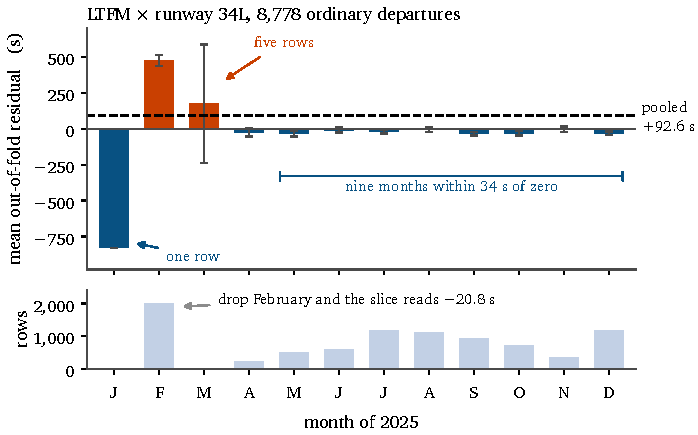
\includegraphics[width=\textwidth]{figures/slice-months.pdf}
  \caption{Monthly mean residual and row count of Istanbul's runway 34L slice. Its pooled +92.6 s survives a permutation null and belongs to one month: February holds 2,000 of its 8,778 rows, January one, and without February the slice reads -20.8 s. Residuals of the twelve-month cross-fit; the sweep, on its own out-of-fold residuals, scored the slice at +76.9 s.}
  \label{fig:7}
\end{figure}

Two months of opposite sign and nine months near zero, and the row counts narrow it further: January is one row and March is five, so the entire pooled mean is February. The pooled mean is real and statistically extreme, and it describes an episodic operational event rather than a property of the airport. A wider null does not change the reading. Residuals cluster, with an intra-cluster correlation of 0.0149 over 3,650 airport-days of 571 rows each, a standard-error inflation of 3.08, and a block permutation over whole airport-days moves the null maximum from 36.07 to 50.63, which the observed 157.7 still exceeds. A slice-discovery procedure therefore needs two calibrations: a permutation null over the whole search, which prices the search, and an out-of-sample split along whatever axis the deployment will cross, which prices the transfer. The null alone was 7.6 RMSE-equivalent seconds too optimistic.

\subsection{Two gates for a committed cell}\label{sec:E.4}

A committed cell replaces the model's prediction on the rows a predicate selects with a fixed hypothesis, for example the schedule copy. When the cell mixes rows of both kinds, the least-squares weight on the hypothesis is $\sum_i p_i D_i^2 / \sum_i D_i^2$ over the rows the cell would change, where $D_i$ is the distance between the two hypotheses and $p_i$ the probability of the first: a rate in which each row counts by the square of how far the commitment moves it, rather than the rate counted over rows. Four commitments, each with its rule fixed in advance, were submitted to the 2026 set, all four having passed the same permutation null. Two paid and two lost. Table~\ref{tab:27} gives each predicate's labelled schedule-copy rate overall, in each half of 2025 (H1, H2) and in its worst month:

\begin{table}[htbp!]
  \centering
  \small
  \setlength{\tabcolsep}{5pt}\renewcommand{\arraystretch}{1.15}
  \caption{Four committed cells and the two gates.}
  \label{tab:27}
  \begin{tabularx}{\linewidth}{>{\raggedright\arraybackslash}Xrrrrrrr}
  \toprule
  \textbf{Predicate} & \textbf{2025 rows} & \textbf{All} & \textbf{H1} & \textbf{H2} & \textbf{Gap} & \textbf{Worst month} & \textbf{2026 gain (s)} \\
  \midrule
  A: one airport, failed join, stand 4xx & 28 & 0.0\% & 0.0\% & 0.0\% & 0.0\% & 0.0\% & +0.2585 \\
  B: eleven total-fallback carriers & 1,805 & 97.7\% & 96.1\% & 98.8\% & 2.7\% & 92.5\% & +0.9790 \\
  C: one carrier & 759 & 81.0\% & 84.6\% & 77.5\% & 7.0\% & 68.3\% & -2.3067 \\
  D: nine deterministic flight numbers & 507 & 99.4\% & 100.0\% & 99.1\% & 0.9\% & 97.1\% & -0.9597 \\
  \bottomrule
  \end{tabularx}
\end{table}

A commits its rows away from the schedule copy, the others toward it. Two gates each reject the loss the other passes.

A temporal split, requiring the rate on the first half of the labelled year to match the second half within five points, rejects C, whose 81.0\% is a mixture and whose halves disagree by 7.0 points. It ranks D the most stable of the three cells whose rate is not zero.

A support-range test, requiring every committed row to sit inside the range of the predicate's own labelled support, rejects D, whose rate was 100.0\% in both window months and at least 99.1\% in each half and which lost because a single committed row sat at a schedule deviation of 12,905 s against a labelled support spanning 600 to 2,884 s, carrying 94\% of $Q$. It passes C, whose rows were all in range.

Both gates certify a rate on the labelled year, and a feed can change between years. A cell of Fiumicino flight numbers that never join a flight plan copied the schedule on 83 of 87 rows delayed by an hour or more in 2025 (95.4\%, steady across the halves), passed both gates, and lost on the 2026 set (226.3833 to 226.4823). The carrier cell of Section~\ref{sec:4.6}, whose 2026 state was read from the scored months' own labelled arrivals, recovered its expected gain (Section~\ref{sec:6.3}); its labelled rows fall in November and December only, so the temporal split could not be applied to it. Where the scored period's labels can show a mechanism's current state, the commitment should rest on them where possible rather than on last year's rate.

\subsection{Pre-registration and adversarial verification}\label{sec:E.5}

The last phase of this work fixed each hypothesis's population, oracle, estimator, submission rule and kill rule in writing before any model for it was fitted, and handed every result to a separate AI agent session, given the scripts and instructed to refute the result by re-running them. Of the first two hypotheses registered this way, one passed and was paid as predicted (\ref{sec:E.1}); the other passed its first test and failed its confirmation on months it had never been read on (\ref{sec:A}). The one that paid had been refused by this work's own pre-submission check, whose bar came from the attenuation estimates of \ref{sec:E.1}; it was submitted on a decision, recorded before the result was known, to override the check. The verifiers overturned or resized several results that had looked positive, the encoding leak of \ref{sec:B} among them, and overturned neither of the two decisions.

Every change of Table~\ref{tab:15} was registered the same way, with a predicted score and a kill line written before submission; seventeen of the twenty-one improved on the best before them. Of the last ten, seven landed near their predicted score or better; one was killed, and two cleared their kill lines at a fraction of their prediction.

\end{document}
